\documentclass{kththesis}


\usepackage{csquotes} % Recommended by biblatex
\usepackage[backend=biber]{biblatex}
\addbibresource{bibliography.bib} % The file containing our references, in BibTeX format
\usepackage{graphicx}
\usepackage{subcaption}
\usepackage[hidelinks]{hyperref}
\usepackage{cleveref}
\usepackage{booktabs}

% My stuff
\graphicspath{{../images/}}
\usepackage{amsmath}
\usepackage{amssymb}
\newcommand{\bibentry}[1]{\parencite{#1}}
\usepackage[disable]{todonotes}
\newcommand{\subsubsubsection}{}


\title{Real-time segmentation of feet on smartphone}
\alttitle{Realtids segmentering av fötter på smartphone}
\author{Axel Demborg}
\email{demborg@kth.se}
\supervisor{Hossein Azizpour}
\examiner{Danica Kragic}
\programme{Master in Computer Science}
\school{School of Electrical Engineering and Computer Science}
\date{\today}


\begin{document}

\listoftodos

% Frontmatter includes the titlepage, abstracts and table-of-contents
\frontmatter

\titlepage

\begin{abstract}
  \todo{This is far to short, we need a why, what, how and result}
  In this work neural networks for real-time semantic segmentation of feet on
  smartphones have been built and evaluated. The models have been trained on a
  dataset consisting of synthetically composited images of feet on a variety of
  floors where the feet have been extracted from 3D-scan data from
  \textit{Volumental's}, the company where the thesis has been performed, foot
  scanner and the floors have been scraped from online images. A secondary
  dataset with real images of feet in natural environments has also been used
  for testing generalization from the synthetic dataset.

  The fastest neural network designed takes \(7.2Mb\) to store, runs at
  \(10fps\) on a 2016 android smartphone without hardware acceleration while
  still producing good segmentations on both datasets.

\end{abstract}


\begin{otherlanguage}{swedish}
  \begin{abstract}
    I det här arbetet har neuronnät för semantisk segmentering av fötter
    byggts och testats. Modellerna har tränats på ett dataset av syntetiska
    bilder av fötter på varierande golv. Fötterna har hämtats från
    3D-skanningsdata från \textit{Volumentals}, företaget där exjobbet har
    utförts, 3d-skanner och golven har hämtats från internet. Ett andra dataset
    med riktiga bilder på fötter har också använts för att se hur modellerna
    generaliserar från den syntetiska datan.

    Det snabbaste nätverket som har designats tar \(7.2 Mb\) att lagra och kan
    köra i \(10fps\) på en androidmobil från 2016 och ger god segementering på
    bägge dataseten.
  \end{abstract}
\end{otherlanguage}

\section*{Acknowledgments}
Firstly I would like to thank my supervisors, Alper Aydemir and Hossein Azizpour for
the help and support they have given me in compleeting this thesis. This would
have been much harder and less fun without you.

I would also like to thank Emil Ernfeldt for his fantastic help with creating and
managing the datasets used in this work as well as for building the monstrosity
of a network that was used as a teacher in some of the experiments.

Further I would like to extend a huge thanks to the entire staff at Volumental whom have made it a joy to go to work
each day, even when my code has just been crashing. It has been a true pleasure to share an office with all of you!


\tableofcontents


% Mainmatter is where the actual contents of the thesis goes
\mainmatter


\chapter{Introduction}
%Semantic segmentation

% For segmentation of human bodies, the problem of classifying each pixel in a
% image, specialized hardware has traditionally been used. \todo{Maybe some more
%   thinking required in this intro?} However with the recent developments in convolutional neural networks
% (CNN) where high quality object segmentation \parencite{BriefHistory} and pose
% estimation \parencite{he2017mask} have been performed from RGB images it should
% be possible to do online segmentation of human bodies with commodity smartphone cameras. An issue
% for mobile deployments of these networks however is their shear size meaning
% that they can't fit in the on-chip SRAM and instead have to reside in the power
% hungry off-chip DRAM making applications up to 100 times more power consuming
% \parencite{han2015learning}. Another issue concerns the computational load of
% the models and means that the networks can't run in real-time on the relatively
% limited processing power of a smartphone. 

% Further issues with supervised methods like these are that they require huge amounts of
% labeled data to train and that generating high quality ground truth data is
% expensive. This is especially true for tasks like semantic segmentation
% where pixel level annotations have to be made for each image and labeling a
% single image is a tedious task, not to mention the thousands required for
% training. 

Segmentation is the problem of partitioning an image into multiple, meaningful
regions, allowing for easier understanding of images. Semantic segmentation
is when the class of the region is also predicted, this problem can also be
formulated as predicting the class of each pixel in an image. These are both
very important problems in computer vision and are relevant for everything from
scene understanding and autonomous driving to synthetic camera effects. Early
approaches utilizing low-level image features to perform segmentation have
recently been outmatched by machine learning models processing the entire image
at once. Deep convolutional neural networks (CNN:s) have been especially
prominent for these tasks.

With these rapid developments, modern smartphones with their high quality
cameras, quite able processors and immense availability have become a sought
after target to run CNN:s on. Deep neural networks are however normally very
large models and tend to require a lot of computation to evaluate. These
requirements are problematic for mobile deployments. Firstly, the large
models can't fit in the on-chip cache and instead have to reside in the power
hungry off-chip DRAM making applications up to 100 times more power consuming
\parencite{han2015learning}. Secondly, the mobile processors can't keep up with
the computational load of the models and hence take seconds to run. This gives
performance far from real-time which is required for smooth operation in many
cases. To address these issues methods for compressing models and designing
streamlined models that can be run in real-time on mobile hardware have been
investigated.

In the intersection of these two lines of research, segmentation and
streamlining of neural networks lies this thesis. The project was performed at
the company \textit{Volumental}, a company specialized in 3D scanning of feet
for custom shoe recommendations. The companies current product is a designated
3D scanner but for the online shopping experience a mobile app with similar
capabilities is required. A first step towards such an application is to create
a model that can reliably perform segmentation of feet in real-time on a
smartphone.

A problem for supervised machine learning methods and deep neural networks in
particular is that they require huge amounts of annotated data for training.
Producing these labeled datasets can be very time-consuming and expensive
especially for image segmentation where producing a single high quality
ground truth frame is a tedious task for a human. Having access to data from
Volumental's dedicated 3D scanner however means that high quality synthetic
datasets can be produced and learned from, reducing the need for manual annotation.

\textit{\textbf{Problem formulation:} To build a system for real-time segmentation of feet that can reliably be run on a
  smartphone and be trained on synthetic data.}
\section{Research Questions}
%\todo{Make this into actual text}
To address these issues this thesis will focus on two research questions:
\begin{enumerate}
\item To what extent can modern neural networks be slimmed down and optimized for
  real-time execution on smartphones?
\item How well does performance from networks trained on synthetic datasets
  transfer to real world data? 
\end{enumerate}
  
\chapter{Background}
\section{Related work}
Convolutional Neural Networks (CNN) were first introduced in 1998
\bibentry{lecun1998gradient} and since then deeper and deeper CNNs have slowly
become the state of the art method for most areas of computer vision. Notably
\emph{AlexNet} \bibentry{krizhevsky2012imagenet} in 2012 proved that that deep
CNNs can be used for high resolution image classification by beating the
previous state of the art \bibentry{sanchez2011high} on the \emph{ImageNet}
classification challenge \bibentry{deng2009imagenet}. To do this \emph{AlexNet},
visualized in \cref{fig:AlexNet}, 
used 60 million parameters and 650,000 neurons. Training of the network was
only made feasible by the use of multiple graphical processing units (GPUs)
\bibentry{krizhevsky2012imagenet}.

\begin{figure}[h]
  \centering
  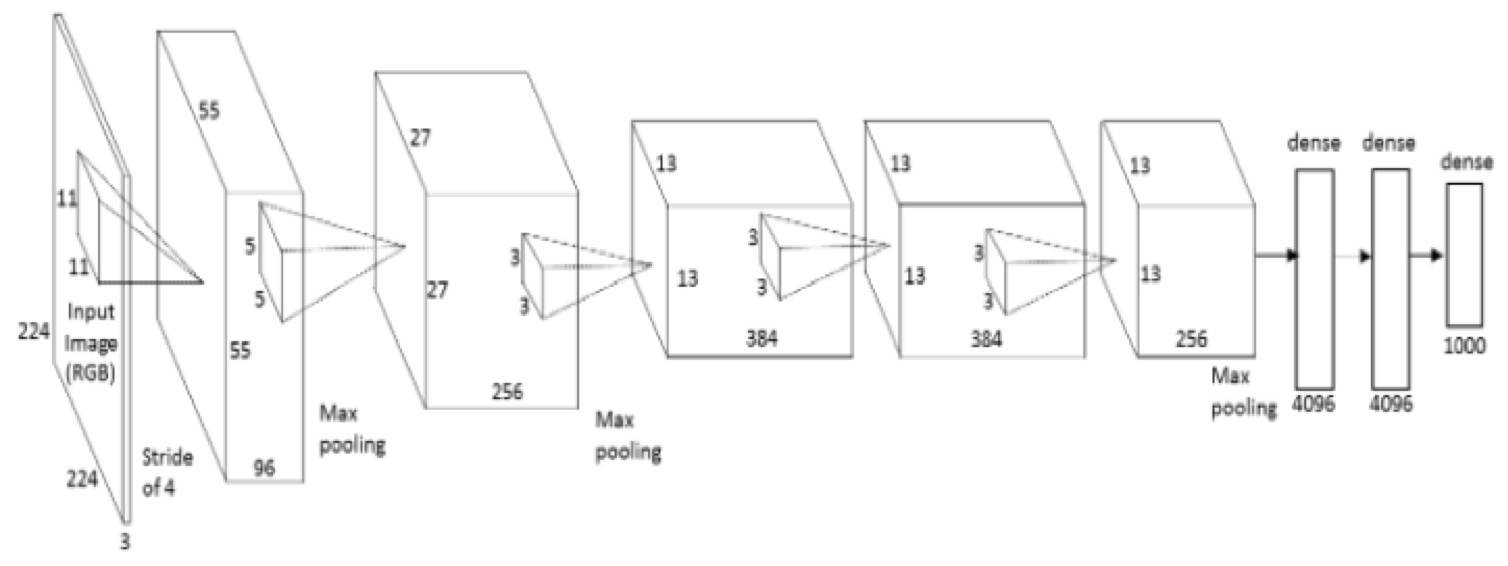
\includegraphics[width=0.7\textwidth]{AlexNet}
  \caption{The architecture of \textit{AlexNet} with its 60 million parameters
    distributed
    in eight layers, five convolutional and three fully connected. Figure from \textcite{krizhevsky2012imagenet}.}
  \label{fig:AlexNet}
  \end{figure}

The following sections will start with a summary of the work that has been done
on extending CNNs for semantic segmentation and related problems like
object detection. This will be followed by a discussion about how these networks
are not suitable for mobile applications. Finally, approaches for compressing
and building networks that can be run on mobile devices will be presented.

\subsection{Semantic segmentation}
In the areas of object detection and semantic segmentation \emph{Regions
  with CNN features} (\emph{R-CNN}) \bibentry{girshick2014rich} 
first showed in that CNNs can be successfully be applied to these fields by
significantly improving over the previous state of the art in object detection
\bibentry{ren2013histograms} After minor modifications matching the
performance of the state of the art in semantic segmentation
\bibentry{carreira2012semantic} with a system not specifically built for the
task. For object detection \emph{R-CNN} works as a hybrid system with
\emph{selective search} \bibentry{uijlings2013selective} producing proposals for
object regions and a CNN, pre-trained on \emph{ImageNet}
\bibentry{deng2009imagenet} and fine-tuned for region classification, generating
fixed length features for each region, finally classifying each region by
running class specific \emph{support vector machines}
\bibentry{boser1992training} on these features, this pipeline is illustrated in \cref{fig:R-CNN}.

\begin{figure}[h]
  \centering
  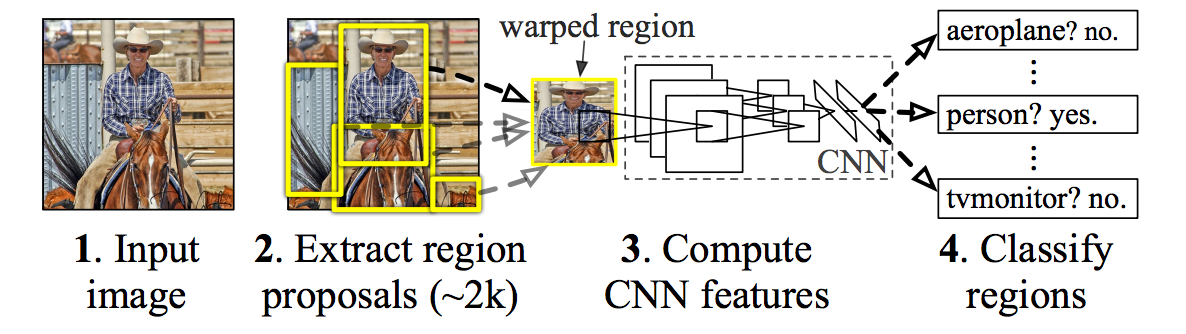
\includegraphics[width=0.9\textwidth]{R-CNN}
  \caption{The object detection pipeline of \textit{R-CNN} which illustrates the
  region proposals from selective search, the computation of CNN features from
  these regions and the final SVM classification. Figure from \textcite{girshick2014rich}.}
  \label{fig:R-CNN}
  \end{figure}

Some issues with \emph{R-CNN}
are that it requires multistage training, training the CNN to give good
features and the SVMs for classification, which is slow. Not only for training
but most notably at inference where one image is processed in 47s.
These problems are addressed with further work resulting in \emph{Fast R-CNN}
\bibentry{girshick2015fast}. In this work the network isn't run once per proposed region but
instead once for the entire image generating a convolutional feature map that
is then pooled with a region of interest (RoI) pooling layer to produce a
feature vector for each region. These feature vectors are then feed into a fully
connected neural network with two sibling output layers that perform both
classification and bounding box refinement in parallel, this architecture is
illustrated in \cref{fig:FastR-CNN}. With these improvements
\emph{Fast R-CNN} achieves faster inference and higher accuracy than its
predecessors and does so with a arguably much more elegant design.

\begin{figure}[h]
  \centering
  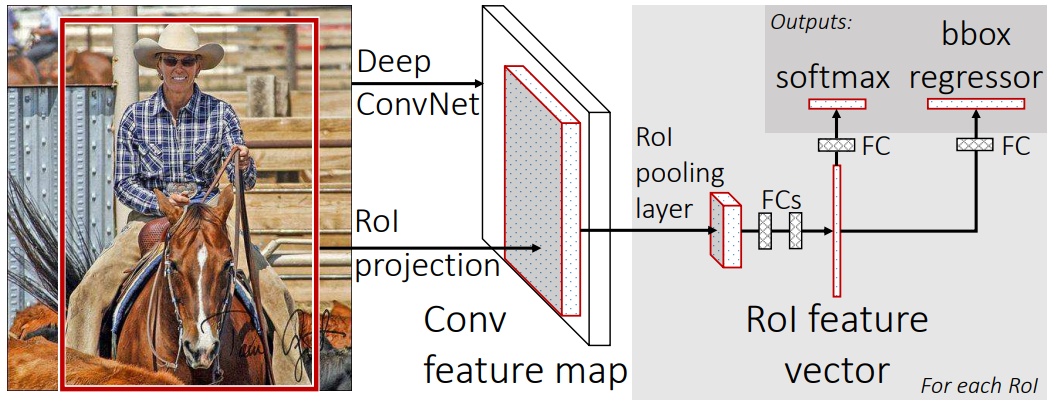
\includegraphics[width=0.7\textwidth]{FastR-CNN}
  \caption{The architecture of \textit{Fast R-CNN} illustrates how the
    convolutional feature map is only calculated once. Figure from \textcite{girshick2015fast}.}
  \label{fig:FastR-CNN}
  \end{figure}

Even though
\emph{Fast R-CNN} improved speed significantly it was nowhere near real-time
performance. Further performance improvements were introduced with \emph{Faster
  R-CNN} \bibentry{ren2015faster} where \emph{selective search} for region
proposals is replaced with Region Proposal Networks. These are fully convolutional neural
networks that take as input the convolutional feature maps introduced in 
\emph{Fast R-CNN}\parencite{girshick2015fast} and outputs region proposals. Since this approach for region
proposals shares most of its computation with the classification network, as illustrated in \cref{fig:FasterR-CNN}, the
region proposals are practically free and frame rates of 5fps are achievable on
a K40 GPU.
The region proposal networks not only speed up computation but also prove to
give better accuracy region proposals and thus raise overall accuracy in the
system as well \bibentry{ren2015faster}.

\begin{figure}[h]
  \centering
  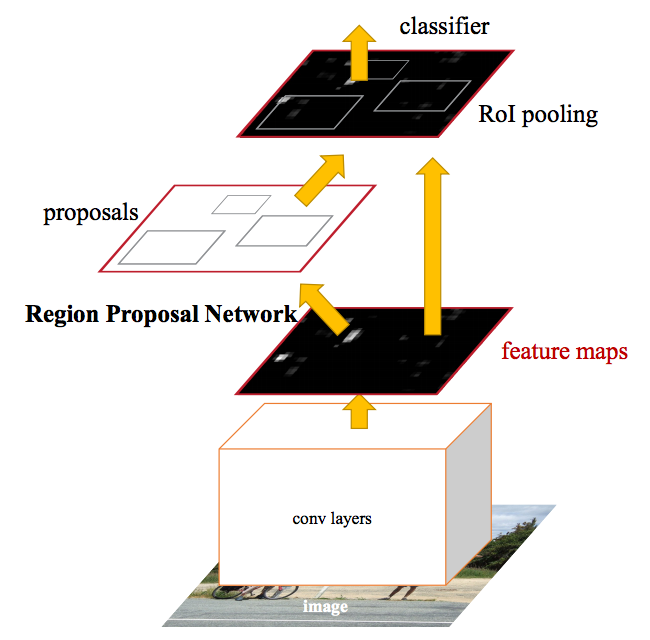
\includegraphics[width=0.5\textwidth]{FasterR-CNN}
  \caption{The architecture of \textit{Faster R-CNN} shows how the feature maps
    are also used for region proposals. Figure from \textcite[]{ren2015faster}.}
  \label{fig:FasterR-CNN}
  \end{figure}

Even further improvements to this
framework was achieved with the introduction of \emph{Mask R-CNN}
\bibentry{he2017mask} which expands upon \emph{Faster R-CNN} by adding a third
branch for a segmentation mask besides the branches for bounding box refinement
and classification making the system able to predict not only the general
bounding box of items in the image but also which exact pixels belong to the
object. Since segmentation is a pixel-by-pixel prediction problem \emph{Mask
  R-CNN} replaces the spatially quantizing RoIPool operation from \emph{Fast
  R-CNN} with a quantization-free layer called RoIAllign. 

\begin{figure}[h]
  \centering
  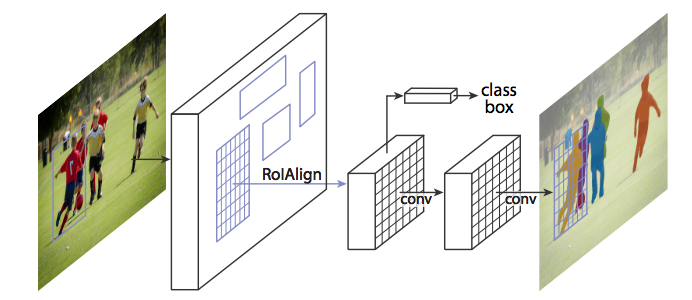
\includegraphics[width=0.5\textwidth]{MaskR-CNN}
  \caption{\textit{Mask R-CNN} adds a branch for segmentation to the body of
    \textit{Faster R-CNN}. Figure from \textcite[]{he2017mask}.}
  \label{fig:AlexNet}
  \end{figure}

Parallel work on semantic segmentation for medical imaging resulted in
\emph{U-Net} \parencite[]{UNet}, a fully convolutional encoder-decoder network.
Here the encoder projects the image into a lower dimensional feature space.
The low dimensional representations are then run through a decoder
network which is architecturally a mirror image of the encoder network but where
the max pooling operations have been replaced with transpose convolutional
layers. Further, the corresponding feature map of the downsampling path is
concatenated to the upsampled features, thus preserving
granularity of the images, see \cref{fig:UNet}. The final layer in the network is a softmax and hence
the outputs are the probabilities of each pixel belonging to each class.
\begin{figure}[h]
  \centering
  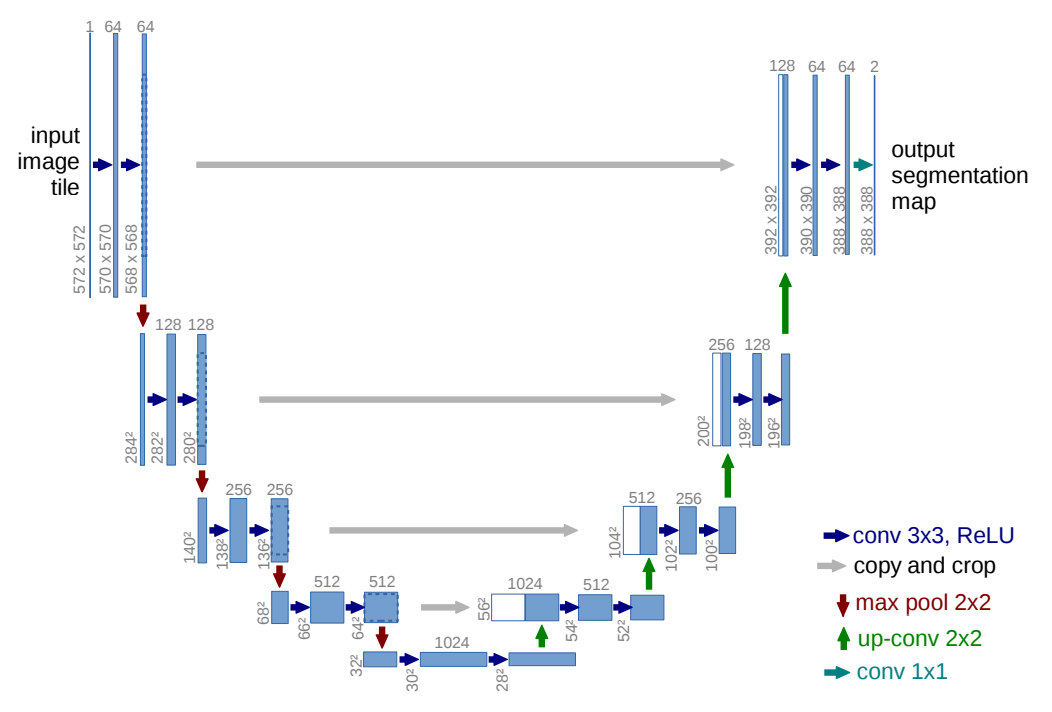
\includegraphics[width=0.9\textwidth]{U-Net}
  \caption{The U-shaped architecture of \textit{U-Net} with skip connections for
    the feature maps in the middle. Figure from \textcite[]{UNet}.}
  \label{fig:UNet}
  \end{figure}

Further work with encoder-decoder structures for segmentation resulted in \emph{SegNet}
\bibentry{badrinarayanan2015segnet}. This network is architecturally very
similar to \textit{U-Net} with the  major differences being how image
granularity is preserved. Instead of concatenating the feature maps like they
looked before max-pooling in the encoding branch to the upsampled feature maps
just the indices of which value was kept in max-pooling is stored in
\textit{SegNet}. This means that one integer, the index of the kept value, is
stored instead of four floats, the values themselves has to be stored for
each cell that max-pool is run over. This reduces the memory footprint of the
network significantly.

\begin{figure}[h]
  \centering
  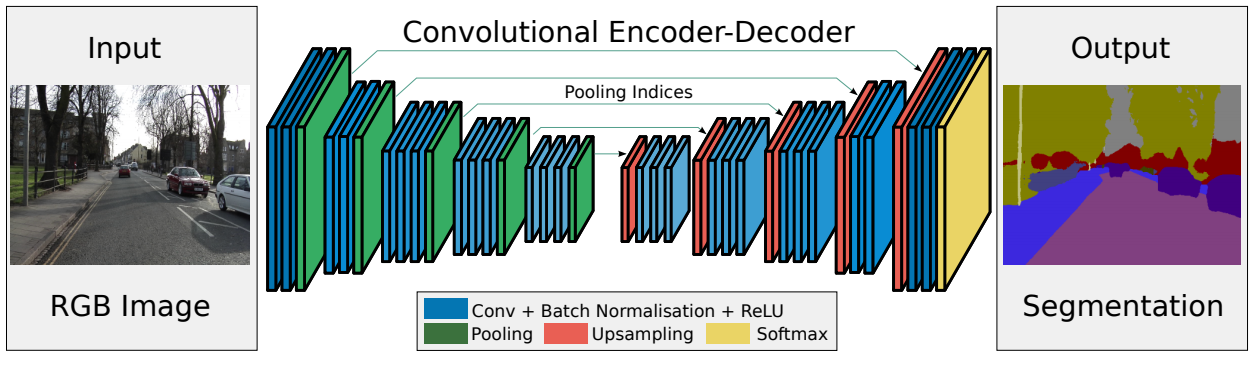
\includegraphics[width=0.9\textwidth]{SegNet}
  \caption{The architecture of \textit{SegNet} illustrating the symmetrical
    encoder-decoder structure. Figure from \textcite[]{badrinarayanan2015segnet}.}
  \label{fig:SegNet}
  \end{figure}

Continued work on segmentation utilizes blocks of so called \emph{DenseNets}
\bibentry{huang2017densely}, CNNs where every layer is connected to every layer
after it, see \cref{fig:DenseNet}, enabling the training of exceedingly deep network architectures by
alleviating the vanishing gradient problem and promoting feature reuse between
the layers.

\begin{figure}[h]
  \centering
  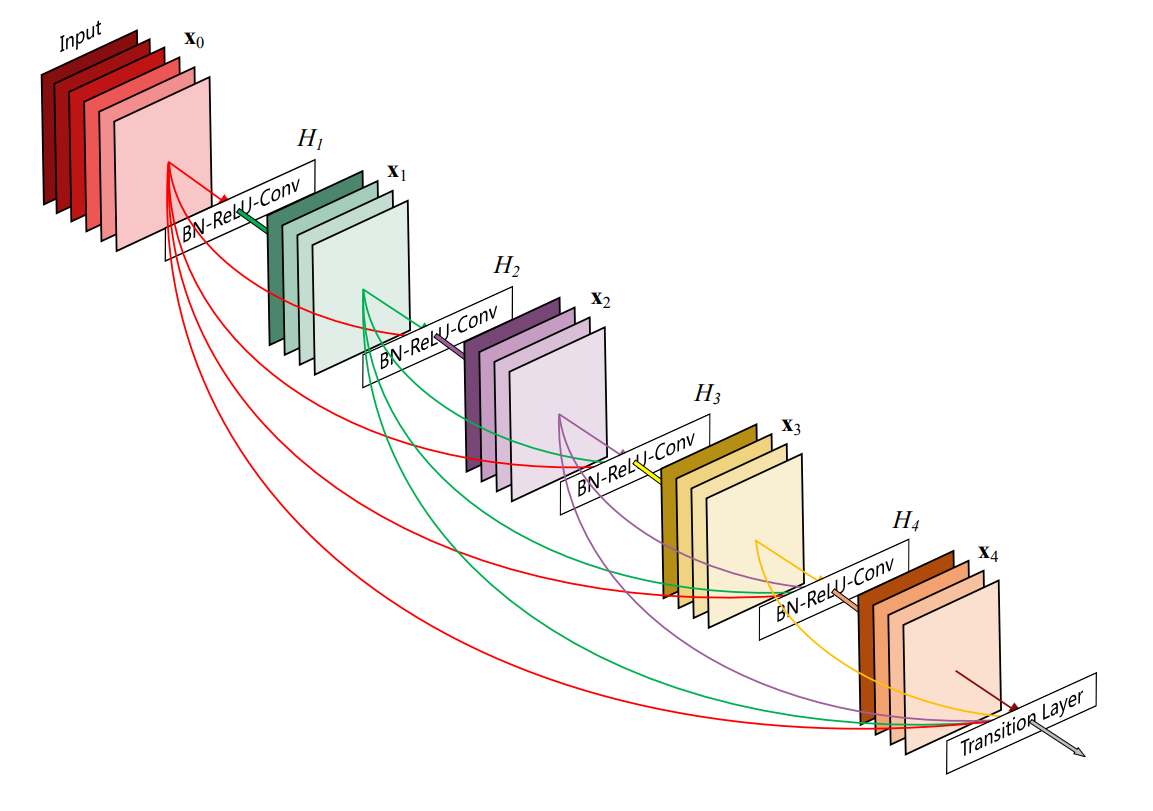
\includegraphics[width=0.5\textwidth]{dense}
  \caption{An example of a \textit{DenseNet} which illustrates how all the
    layers are connected. Figure from \textcite[]{huang2017densely}.}
  \label{fig:DenseNet}
  \end{figure}

\textcite{jegou2017one} use these \emph{DenseNets} in a very deep encoder-decoder
structure where skip connections, as seen in \cref{fig:Tiramisu}, restore image granularity during upsampling the
state of the art in image segmentation has been pushed even further while still reducing the amount of parameters required
for the models by a factor 10 as compared to the previous state of art. 

\begin{figure}[h]
  \centering
  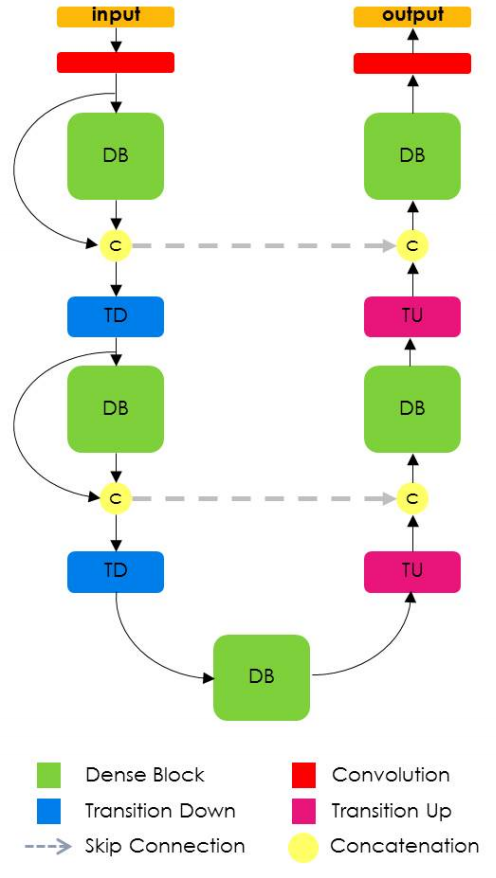
\includegraphics[width=0.3\textwidth]{Tiramisu}
  \caption{The architecture of \textit{One Hundred Layers Tiramisu} where
    DenseNets are used for segmentation. Figure from \textcite[]{jegou2017one}.}
  \label{fig:Tiramisu}
  \end{figure}

  \subsection{Network compression}
Despite their impressive performance on a wide range of problems neural networks
are still prohibited from running locally on mobile devices with slow
processors, limited power envelopes or limited memory due to their large size
and big computational load. For example modern neural networks can't fit on the
on-chip SRAM cache of mobile processors and instead have to reside in the much more power hungry
off-chip DRAM memory making applications up to 100 times more power consuming
\bibentry{han2015learning}. Regarding inference speed modern networks
for object segmentation \bibentry{he2017mask} run at 5fps. That however is on high
performance GPUs meaning that real-time performance on mobile devices is still
largely intractable. Due to
these limitations applications of neural networks for mobile use cases are
either to forced give up on state of the art performance or to be run on
off-site servers which requires steady network connections and incurs latency,
both of which may be intolerable for real-time mobile applications, self driving
cars and robotics \bibentry{jin2014flattened}. However work on understanding the
structure of the learned weights in neural networks
\bibentry{denil2013predicting} has showed that there is significant redundancy
in the parameterization of several deep learning models and that up to 95\% of
weights in networks can be predicted from the remaining 5\% without any drop in
accuracy. This indicates that models can be made much smaller while still
maintaining performance and several such approaches for squeezing high
performance networks into small memory footprints and computational loads have
been proposed. The most prominent approaches will be presented in the following
sections.  

\subsubsection{Quantization of weights}
Modern neural networks are usually based on 32-bit floating point
representations of parameters. It has been shown however that networks are quite
resilient to noise and even that some noise can improve training
\bibentry{murray1994enhanced}. Since reduced precision variables can be modeled
as noise this means that networks can be compressed by changing to a less
accurate format without any loss in performance. This can be done either by
reducing the bit accuracy after training \bibentry{vanhoucke2011improving}  or
by doing the entire training in reduced accuracy \bibentry{hubara2016quantized}
\bibentry{gupta2015deep}. The benefits of using a reduced format like this for
representation is not only that the models take less space but also that the
individual multiplications become cheaper and hence the networks run faster. 

\subsubsection{Weight sharing}
One of the most direct approaches for removing the redundancy in parametrization
from neural networks is by forcing the networks to share weights between
different connections. This is precisely what \emph{HashedNets}
\bibentry{chen2015compressing} does by fixing the amount of weights \(K^l\) that
are to be used in each layer making the weights \(\vec{w^l} \in
\mathbb{R}^{K^l}\) and using hashing functions to map each element in the
virtual weight matrices \(V_{ij}^l\) to one of these weights \(V_{ij} =
w_{h(i,j)}\) with \(h()\) being a hashing function. With the weight matrices
defined in this fashion \emph{HashedNets} can be trained like normal networks
with the gradients with respect to the weights calculated from the gradients
with respect to the virtual matrices as  
\[ \frac{\partial\mathcal{L}}{\partial w_k^l} = \sum_{ij} \frac{\partial\mathcal{L}}{\partial V_{ij}^l}\frac{\partial V_{ij}^l}{\partial w_k^l} \]
This method gave a compression of about 20 times before any notable loss in
accuracy was introduced during tests on variations of the MNIST dataset which
seems to agree very well with the results from \bibentry{denil2013predicting}. 

Other notable work focuses on the use of k-means clustering to cluster the
weights in networks after training \bibentry{gong2014compressing}, this proves
to work very well and manages to compress the models with a factor 16 with no
more than a 0.5\% drop in classification accuracy on the ImageNet dataset.
Further work in this area explores the effects of pruning away low-weight
connections and iterative retraining of the pruned networks
\bibentry{han2015learning}. This lets the authors compress models with a factor
9 - 13 without any loss in performance while getting sparser weight matrices
that could potentially speed up calculations. These two lines of research,
clustering and pruning, where merged into a single framework called \emph{deep
  compression} \bibentry{han2015deep} where a three stage approach is taken to
model compression. First low-weight connections are pruned away and the network
is retrained to compensate for this, in the second stage k-means clustering is
performed on the weights and again the network is retrained to make the clusters
take the most useful values, finally Huffman coding
\bibentry{van1976construction} is used to reduce the storage required for the
weights. This process is illustrated in \cref{fig:DeepCompression} and it allows \emph{deep compression} to compress networks with a
factor 35 without any loss in accuracy. Despite these very impressive results
however \emph{deep compression} comes with a major drawback, it can't be run
efficiently in its compressed form and the full weight matrices have to be
rebuilt at inference time to use the models on commodity hardware. To alleviate
these problems hardware has been designed that can perform prediction directly
from the compressed models. This so called \emph{efficient inference engine}
\bibentry{han2016eie} would enable inference 13 times faster than GPU while
being 3400 times more energy efficient.  

\begin{figure}[h]
  \centering
  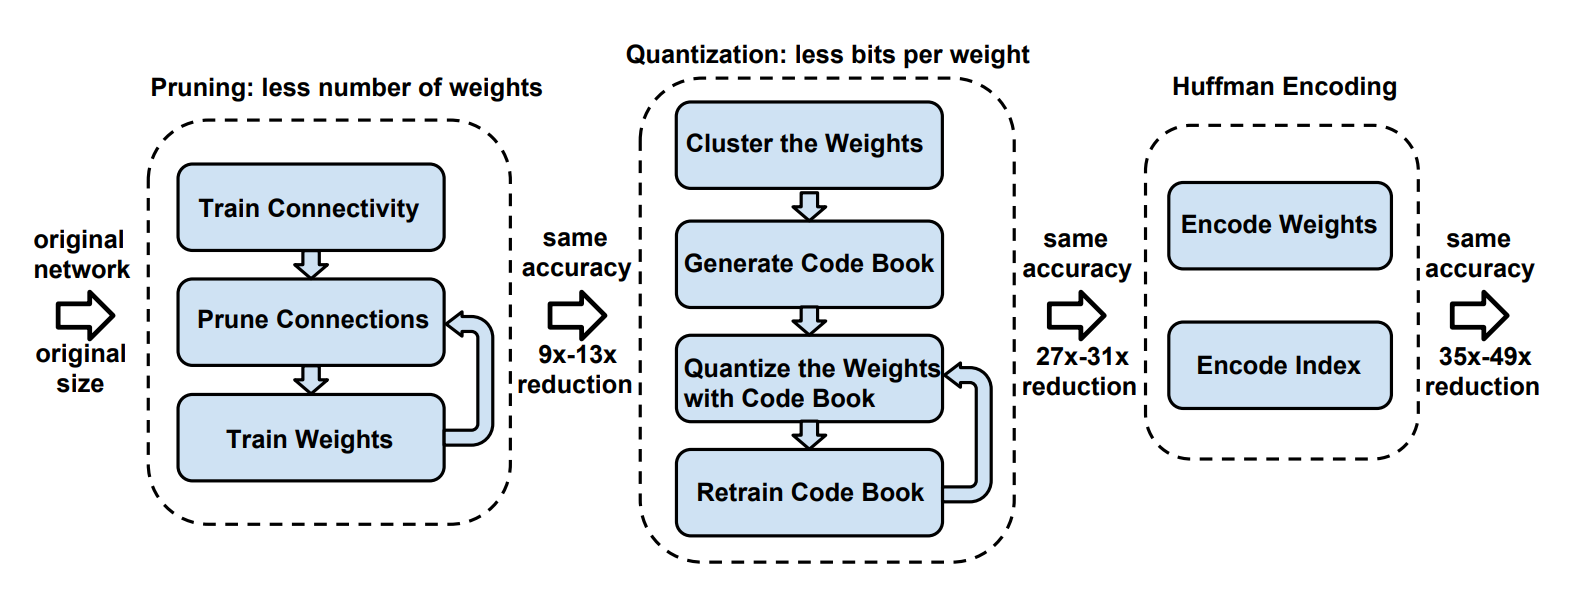
\includegraphics[width=0.9\textwidth]{DeepCompression}
  \caption{The compression pipeline of \textit{deep compression}. Figure from \textcite[]{han2015deep}.}
  \label{fig:DeepCompression}
  \end{figure}

\subsubsection{Student-teacher learning}
Student-teacher learning is a type of model compression where a smaller and/or
faster to compute \emph{student} network is trained by making it learn the
representations learned by a larger \emph{teacher} network. This idea was first
introduced for compressing ensemble models produced by \emph{Ensemble Selection}
\bibentry{caruana2004ensemble} which consist of hundreds of models of many
different kinds, support vector machines, neural networks, memory based models,
and decision trees into a single neural network \bibentry{bucilua2006model}.
This work leverages the neural networks property of being universal
approximators \bibentry{cybenko1989approximation}, meaning that given
sufficiently much training data and a big enough hidden layer a neural network
can learn to approximate any function with arbitrary precision. This is done by not directly
training the student network on the relatively limited labeled training data
available but instead on large amounts of pseudo random data that has been given
labels by first being passed through the large teacher ensemble. This
compression technique yielded student networks up to 1000 times smaller and 1000
times faster to compute than their ensemble teachers with a negligible drop in accuracy
on some test problems \parencite{bucilua2006model}. 

%Further work on student-teacher learning experiments with why deep neural
%networks usually perform better than shallow ones, even when they have the same
%amount of parameters.
Further work on student-teacher learning investigates why slow to compute, deep
neural networks perform better than their shallower and faster siblings, even when
the amount of parameters is the same between them.
This was done by training shallow student models to mimic
deep teachers \bibentry{ba2014deep}. The work introduces two major modifications
that make training of these student models feasible. Firstly, the student model
isn't tasked with just recreating the same label as the teacher but also the
same distribution which is achieved by regressing the student to the logits, log
probability, values of the teacher as they were before softmax. Getting
predictions from the student is then achieved by adding a softmax layer to the
end of it after training. Second, a bottleneck linear layer is added to the
network to speed up training. With these modifications the authors were able to train
flat neural networks for both the TMIT and CIFAR-10 datasets with performance
closely matching that of single deep networks. Continued analysis of flat
networks however shows that depth and convolutions are critical for getting good
performance on image classification datasets \bibentry{urban2016deep}.
Empirically this claim is supported by training state of the art, deep,
convolutional models for classification on the CIFAR-10 dataset and then
building an ensemble of such models using that as a teacher for shallow
students. The student models were then compared to deep convolutional benchmarks
that were not trained in a student-teacher fashion. To make sure that the
networks were all performing to the best of their abilities and thus making the
comparison fair Bayesian hyperparameter optimization
\bibentry{snoek2012practical} was used. Through this thorough analysis it was
shown that shallow networks are unable to mimic the performance of deep networks
if the number of parameters is held constant between them, these findings are
also in agreement with the theoretical results that the representational
efficiency of neural networks grows exponentially with the number of layers
\bibentry{liang2016deep}. 

\subsubsubsection{Distillation}
Improvements to the student-teacher learning method have been proposed where the
student is tasked with minimizing the weighted average of the cross-entropy
between its own output and the teacher output when the last layer is softmax
with increased temperature, yielding softer labels, and the cross-entropy
between the student output and the correct labels when they are available. This
framework is called \emph{Distillation} \bibentry{hinton2015distilling} and
proves to work very well for transferring of information from teacher to
student. The framework is demonstrated by training a student model with only
13.2\% test error on the MNIST dataset despite only having seen 7s and 8s during
its own training. These results mean that distillation manages to transfer
knowledge about how a 6 looks from the teacher to the student by only telling it
to what degree different 7s and 8s don't look like 6s. 

\subsubsubsection{FitNets}
Continued work led to the creation of \emph{FitNets}
\bibentry{romero2014fitnets} which goes in the opposite direction to previous
attempts at student architectures and instead proposes very deep but thin
students. To enable learning in these deep student networks a stage-wise
training procedure is used. In the first stage intermediate layers in the
teacher and student networks are selected, these are called \emph{hint} and
\emph{guided} layers respectively. The guided layer in the student is then
tasked to mimic the hint layer in the teacher through a convolutional regressor
that compensates for the difference in number of outputs between the networks,
this procedure gives a good initialization for the first layers in the student
and allows for it to learn the internal representations of the data from the
teacher. The second stage of training is then distillation as described above
but with the small addition that the weight of the loss against the teacher is
slowly annealed during training. This annealing allows for the student to lean
heavily on the teacher for support in early stages of training and learn samples
which the even the teacher struggles with towards the end of its training. Using
this approach the \emph{FitNets} manage to produce predictions at the same level
or in some cases even better than models with 10 times more parameters. The
training procedure is illustrated in \cref{fig:FitNet}.

\begin{figure}[h]
    \centering
    \begin{subfigure}[b]{0.3\textwidth}
        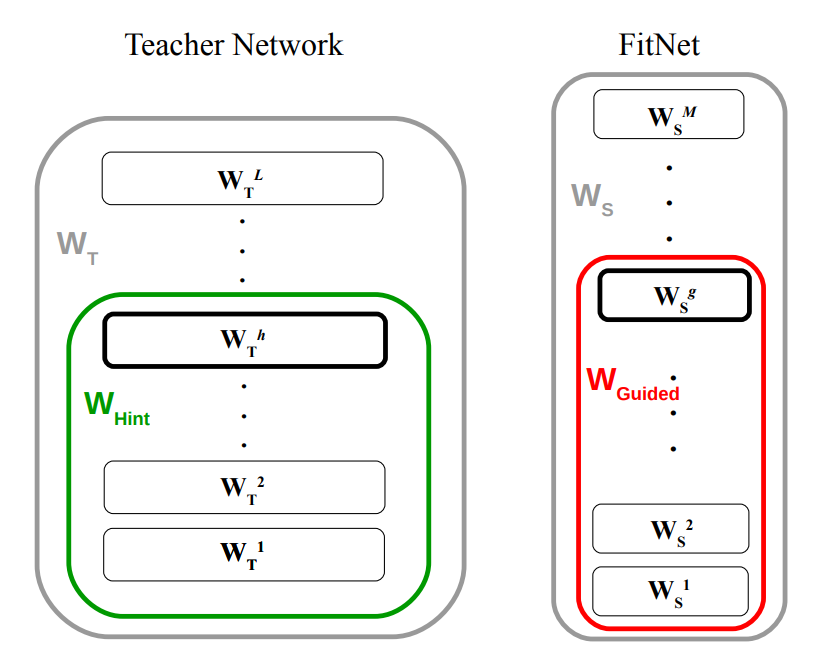
\includegraphics[width=\textwidth]{FitNet_A}
        \subcaption{The student and teacher networks}
    \end{subfigure}
    ~ %add desired spacing between images, e. g. ~, \quad, \qquad, \hfill etc. 
      %(or a blank line to force the subfigure onto a new line)
    \begin{subfigure}[b]{0.3\textwidth}
        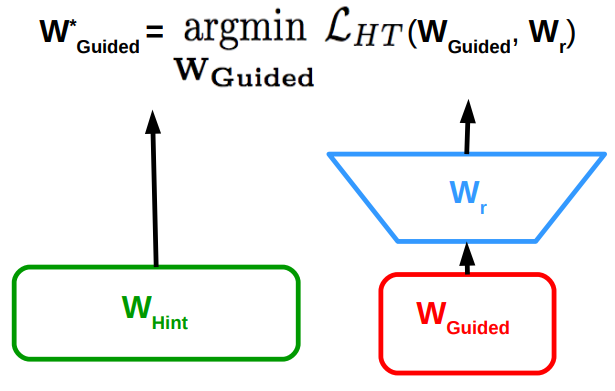
\includegraphics[width=\textwidth]{FitNet_B}
        \subcaption{The initial training of the guided layers in the student.}
      \end{subfigure}
    ~
    %add desired spacing between images, e. g. ~, \quad, \qquad, \hfill etc. 
    %(or a blank line to force the subfigure onto a new line)
    \begin{subfigure}[b]{0.3\textwidth}
        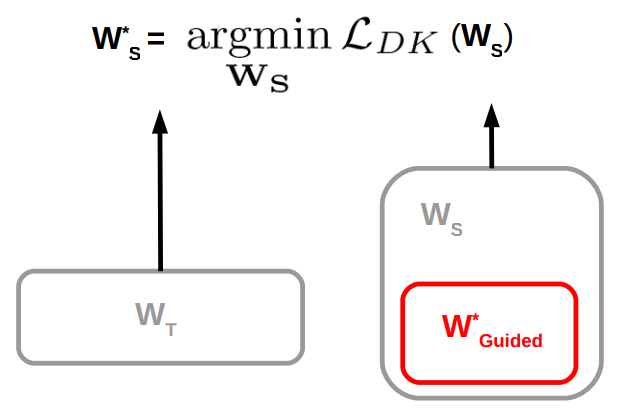
\includegraphics[width=\textwidth]{FitNet_C}
        \subcaption{The final distillation training of the entire student.}
      \end{subfigure}
      \caption{The training procedure for \textit{FitNets}. Figures from \textcite[]{romero2014fitnets}.}\label{fig:FitNets}
      \label{fig:FitNet}
\end{figure}

\subsubsubsection{Attention transfer}
Some more recent work \bibentry{zagouruyko2017paying} builds upon the ideas from
\emph{FitNets} with not only letting the students mimic the output of teachers
but also some intermediary representations. Unlike the way it is done in
\emph{FitNets} however the student is not tasked with reconstructing the exact
activations of the teacher in the intermediate layers but instead the attention
maps, regions in the image that the teacher uses to make its predictions, and
thus teaches the student where to look. A few different methods for calculating
these attention maps are proposed in the paper but notable is that they are all
non parametric meaning that no extra layers of convolution have to be learned to
make the student attention maps comparable to the ones from the teacher. This
attention transferring approach proves to give good results on a number of
difficult datasets including \emph{ImageNet} and is also shown to work well
together with distillation. 

\begin{figure}[h]
  \centering
  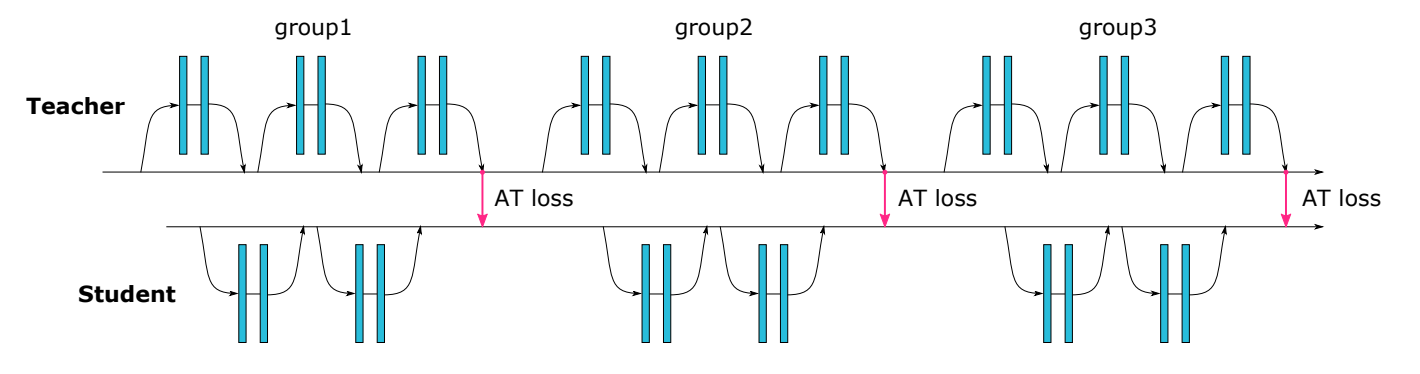
\includegraphics[width=0.9\textwidth]{AttentionTransfer}
  \caption{Illustration of \textit{Attention transfer} showing the tight bond
    between teacher and student during training. Figure from \textcite[]{zagouruyko2017paying}.}
  \label{fig:AttentionTransfer}
\end{figure}

\subsubsection{Optimized convolutions}
Another orthogonal approach for compression is to optimize the convolutional
layers themselves making them require less parameters or less computation to
perform their tasks but still keep as much as possible of their representational
power. One of the simplest things that can be done here is to replace single
layers of \(N \times N\) convolutional filters with two layers with \(N \times
1\) and \(1 \times N\) filters respectively, this reduces the amount of
parameters that have to be stored per channel from \(N^2\) to \(2N\) and the
amount of multiplications that have to be made scale in the same way. These
so called asymmetrical convolutions have seen successful use in inception models
\bibentry{szegedy2016rethinking}.  
Other variations on the convolutional operator that help compress the networks
are dilated convolutions \bibentry{yu2015multi} where an exponentially expanding
receptive field is achieved without the need for any extra parameters. There
have also been some promising results from \emph{depthwise separable
  convolutions} where the convolution is factored into a depthwise convolution
followed by a pointwise \(1 \times 1\) convolution reducing the computational
load with a factor \(8\) to \(9\) for \(3 \times 3\) convolutional kernels
\bibentry{howard2017mobilenets}. This scheme was introduced in
\bibentry{sifre2014rigid} and has since seen been successfully used in
\emph{Inception} models \bibentry{ioffe2015batch}.  


\begin{figure}[h]
    \centering
    \begin{subfigure}[b]{0.3\textwidth}
        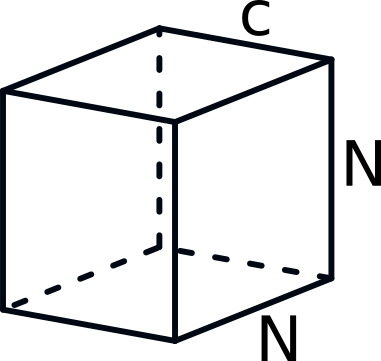
\includegraphics[width=\textwidth]{conv}
        \subcaption{Normal}
    \end{subfigure}
    \qquad %add desired spacing between images, e. g. ~, \quad, \qquad, \hfill etc. 
      %(or a blank line to force the subfigure onto a new line)
    \begin{subfigure}[b]{0.45\textwidth}
        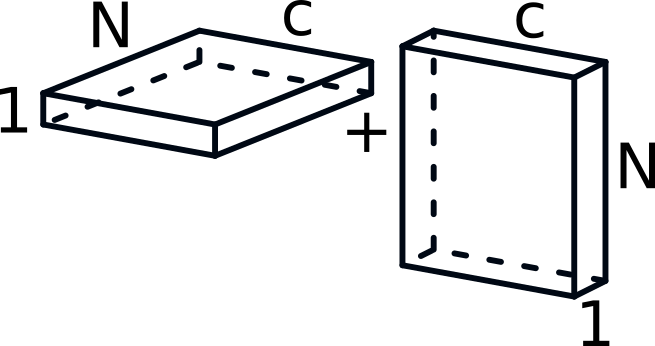
\includegraphics[width=\textwidth]{assymConv}
        \subcaption{Asymmetrical}
      \end{subfigure}

      \begin{subfigure}[b]{0.45\textwidth}
        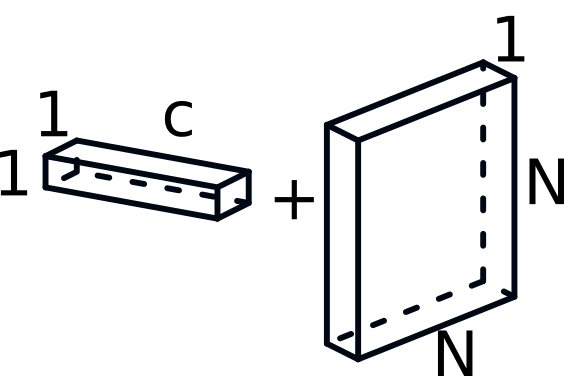
\includegraphics[width=\textwidth]{separable}
        \subcaption{Depthwise separable}
    \end{subfigure}
    \qquad %add desired spacing between images, e. g. ~, \quad, \qquad, \hfill etc. 
      %(or a blank line to force the subfigure onto a new line)
    \begin{subfigure}[b]{0.4\textwidth}
        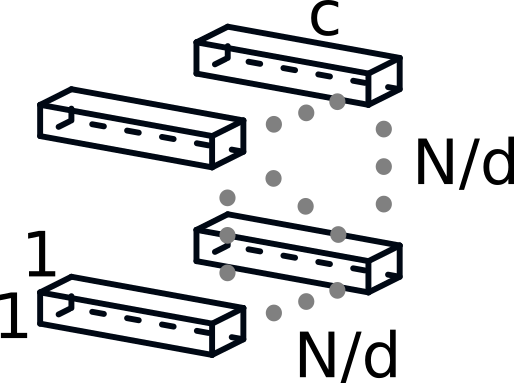
\includegraphics[width=\textwidth]{dilated}
        \subcaption{Dilated}
      \end{subfigure}
      \caption{Visualization of the shapes of the weight matrices to produce one
        feature map for each of the types of convolution. All in the case of a \(N \times N\) filter
        with \(c\) channels. The dilation factor \(d\) corresponds to how
        sparsely the dilated convolutions are applied.}\label{fig:Convs}
\end{figure}

\subsubsection{Streamlined architectures}
\emph{SqueezeNet} \bibentry{iandola2016squeezenet} presents a different take on
how to get smaller models in that it rather optimizes the architecture of the
network than any of the constituent parts, this approach gives a network with
\emph{AlexNet} performance but with 50 times fewer parameters than 
\emph{AlexNet}. This is done by focusing on the usage of \(1 \times 1\)
convolutional filters, reducing the amount of channels that go in to the larger
filters and by holding out on downsampling so that feature maps are kept large
through the network. It was also proven that these results were orthogonal from
compression by running the SqueezeNet through the \emph{deep compression}
framework \bibentry{han2015deep} and getting further 10 times compression with
out accuracy loss. 

\emph{MobileNets} \bibentry{howard2017mobilenets} combine these two approaches,
utilizing both \emph{depthwise separable convolutions} and a heavily optimized
architecture to build networks specially suited for mobile vision applications.
In doing so \emph{MobileNets} also introduce two hyper-parameters,
\emph{width-multiplier} and \emph{resolution-multiplier} that help design models
with a optimal trade off between latency and precision given the limitations of
the available hardware. 

Another network specially designed for real-time segmentation on mobile devices
is \emph{ENet} \bibentry{paszke2016enet}. Here dilated convolutions are used
together with asymmetrical convolutions to give a large receptive field without
introducing that many parameters. The network is built as an encoder-decoder
network but with a much smaller decoder, the argument behind this being that
decoder should simply upsample the output while fine-tuning the details which
should be a simpler task than the information processing and extraction that the
encoder is performing. Attention has also been payed to quickly downsampling the
feature maps which saves on computation but then not downsampling so
aggressively after that, keeping much of the spatial information in the images.
Together these improvements give a network that performs on par with
\emph{SegNet} but that requires 79 times fewer parameters and is 18 times faster
at inference. 
%\todo{Need to talk a bit about LinkNet here}

An other modern network architecture that has been specifically designed for fast and
efficient segmentation is \textit{LinkNet}
\parencite{chaurasia2017linknet}. Here residual blocks \parencite{residual} are used to produce a
state of the art network which can process high resolution frames at almost 10
fps. To maintain image granularity skip connections are used, these can be seen
in \cref{fig:LinkNet}.

\begin{figure}[h]
  \centering
  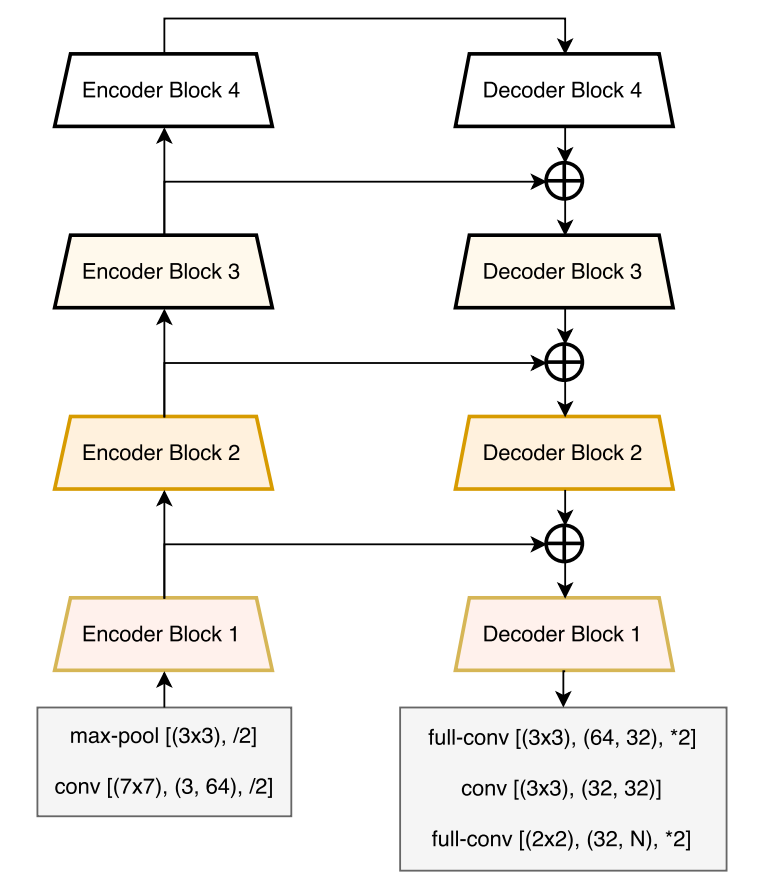
\includegraphics[width=0.45\textwidth]{LinkNet}
  \caption{Architecture of \textit{LinkNet}. Figure from \textcite{chaurasia2017linknet}.}
  \label{fig:LinkNet}
\end{figure}


\chapter{Method} \label{chap:method}

\todo{Add some sort of graph or table detailing the different approches here}
In this project we will try and build a model for real-time segmentation of feet
on a smartphone. Since a system that is deployable right now is required,
compression approaches like deep compression that need custom hardware to be
fully utilized are out of the question. Instead, focus will be placed on how
the highly streamlined architectures like MobileNets and LinkNet can be used and
modified to produce give the required performance. The effectiveness of
student-teacher learning in these models will also be evaluated by training the
networks using knowledge distillation from a big segmentation network previously
designed at Volumental. Here distillation is preferred over more recent
approaches like FitNets or attention transfer since the available teacher was
not specifically designed to a teacher and finding layers suitable for hinting or
transferring attention maps from is hence a problem in it self and outside the
scope of this work.\todo{expand this and give an outline of the method section}

\section{Pipeline}
To train models for segmentation datasets with known segmentations are used. The
images are augmented to artificially expand the available training data and the
augmented image is feed into the the model. The resulting predicted segmentation
is compared to the ground truth and from this a loss is calculated using which
the parameters in the models can be updated. This pipeline is presented in
\cref{fig:pipeline}. The datasets used in this project along with the data
augmentation used and the different loss functions and CNN models tested will be
presented in the following sections.

\begin{figure}[h]
  \centering
  \includegraphics[width=0.85\textwidth]{pipeline}
  \caption{The data pipeline for training and predicting with the model.}
  \label{fig:pipeline}
\end{figure}

\section{Data}
Two datasets of segmented feet were used for the experiments.

Firstly a dataset where images and 3D-models where extracted from
\textit{Volumental's}
3D-scanner and composited with floor images scraped from the internet to create
synthetic images of feet on normal floors. This process is illustrated in \cref{fig:process_synthetic}.
This dataset is called
\textit{synthetic} and is divided into training, validation and test sets with
43896, 12960 and 14168 images respectively. The different sets have been
constructed to ensure that there is no overlap of floors or feet between them.
Example images from this dataset can be seen in \cref{fig:data_synthetic}. Here
the training set is directly used for training, the validation set is used for
hyperparameter optimizations and to track overfitting during training, and
finally the held out test set is used for evaluating the performance of the
models after training.

\begin{figure}[h]
    \centering
    \begin{subfigure}[b]{0.45\textwidth}
        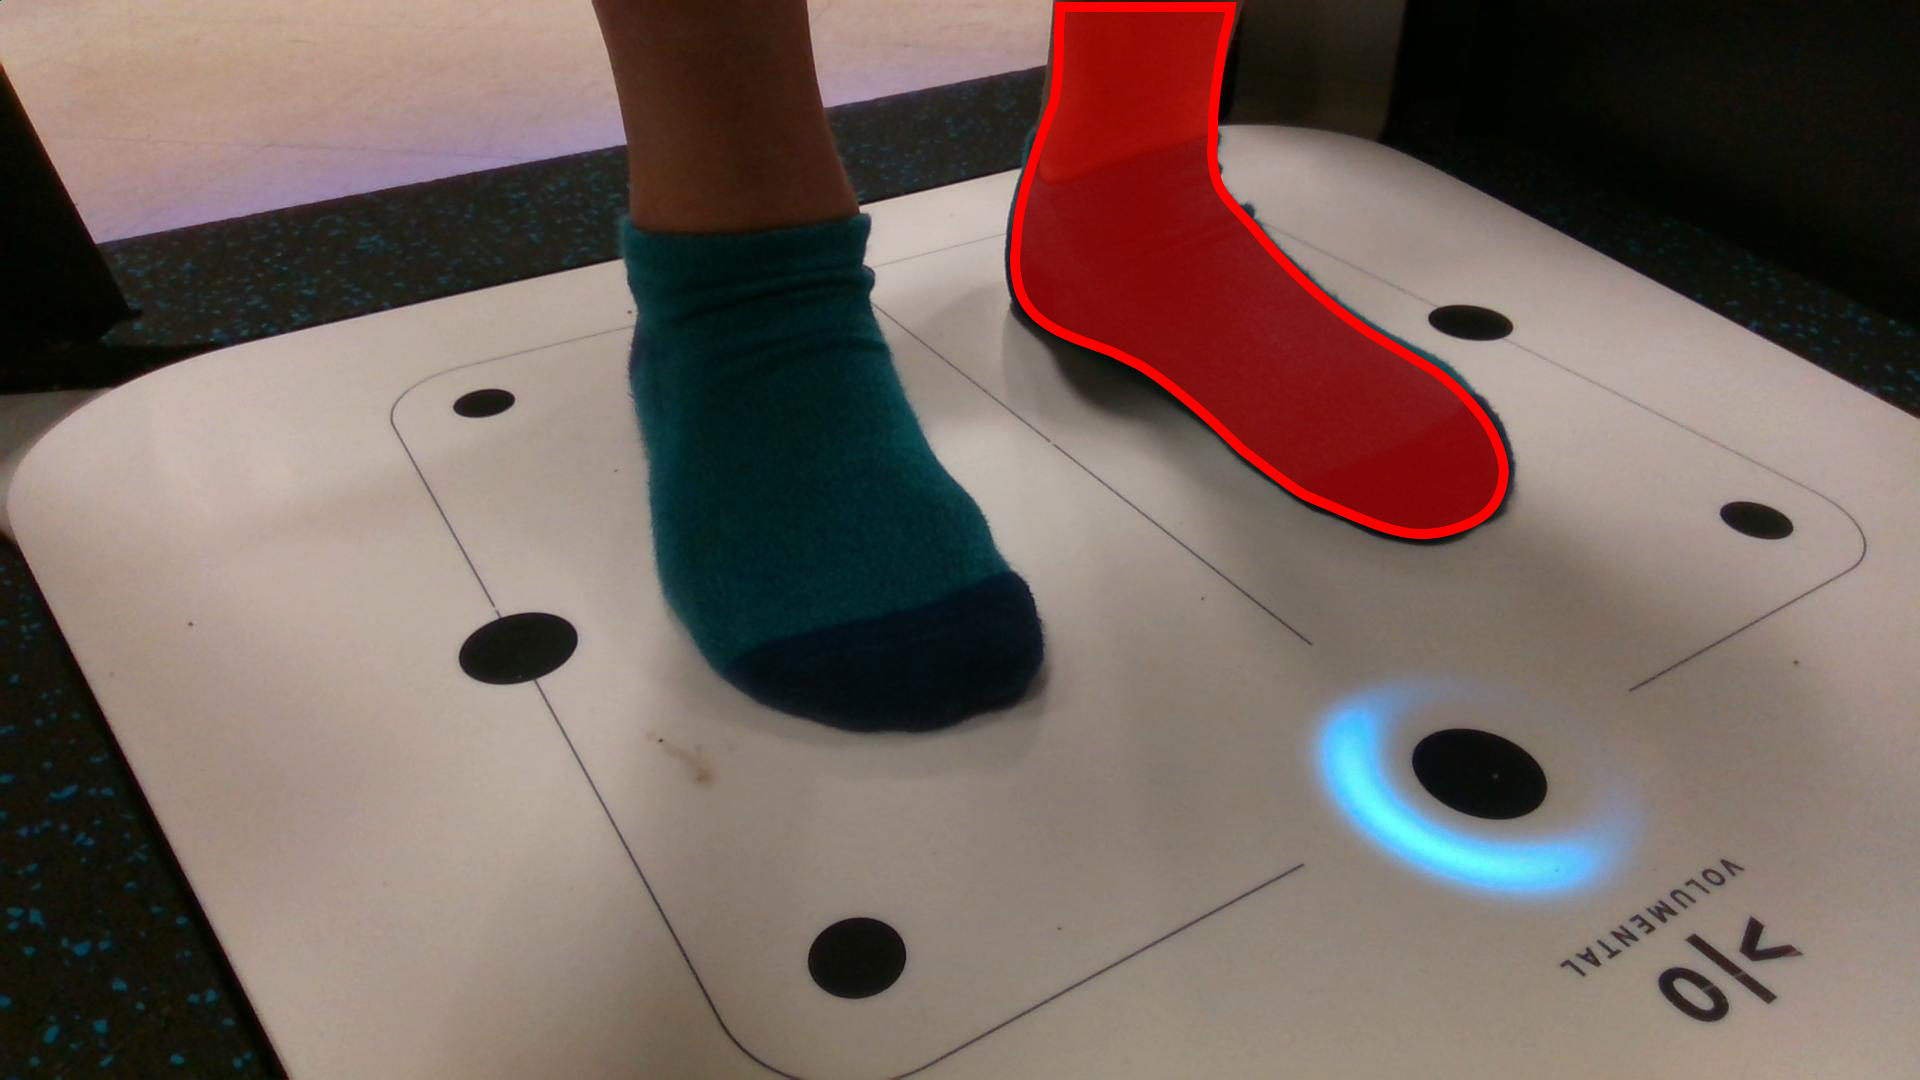
\includegraphics[width=\textwidth]{on_scanner}
        \caption{The foot on the scanner}
        \label{fig:on_scanner}
    \end{subfigure}
    ~ %add desired spacing between images, e. g. ~, \quad, \qquad, \hfill etc. 
      %(or a blank line to force the subfigure onto a new line)
    \begin{subfigure}[b]{0.45\textwidth}
        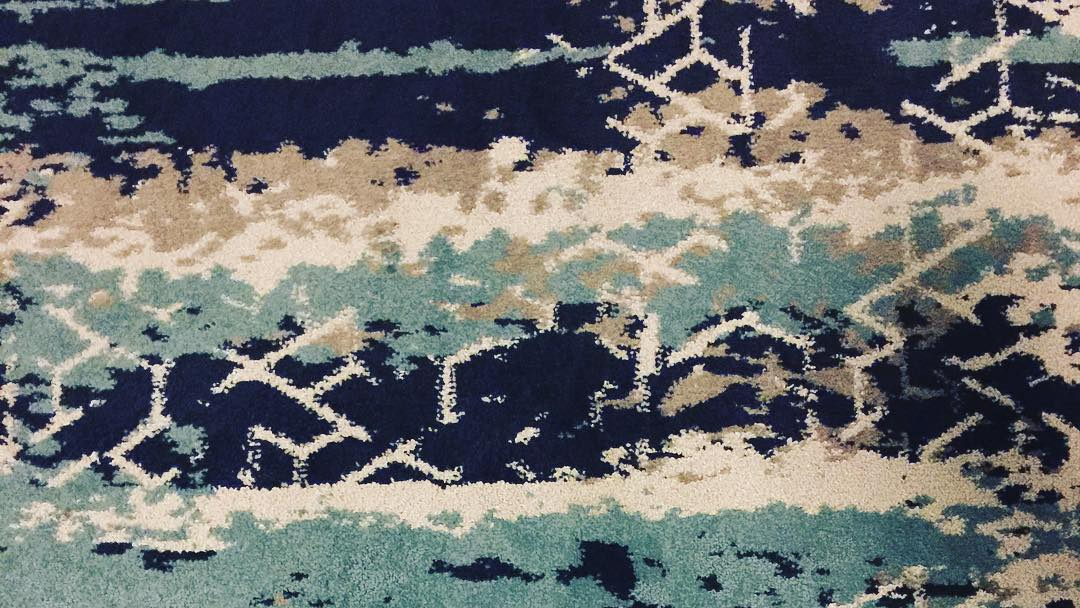
\includegraphics[width=\textwidth]{floor}
        \caption{Floor texture}
        \label{fig:texture}
      \end{subfigure}
      
    %add desired spacing between images, e. g. ~, \quad, \qquad, \hfill etc. 
    %(or a blank line to force the subfigure onto a new line)
    \begin{subfigure}[b]{0.45\textwidth}
        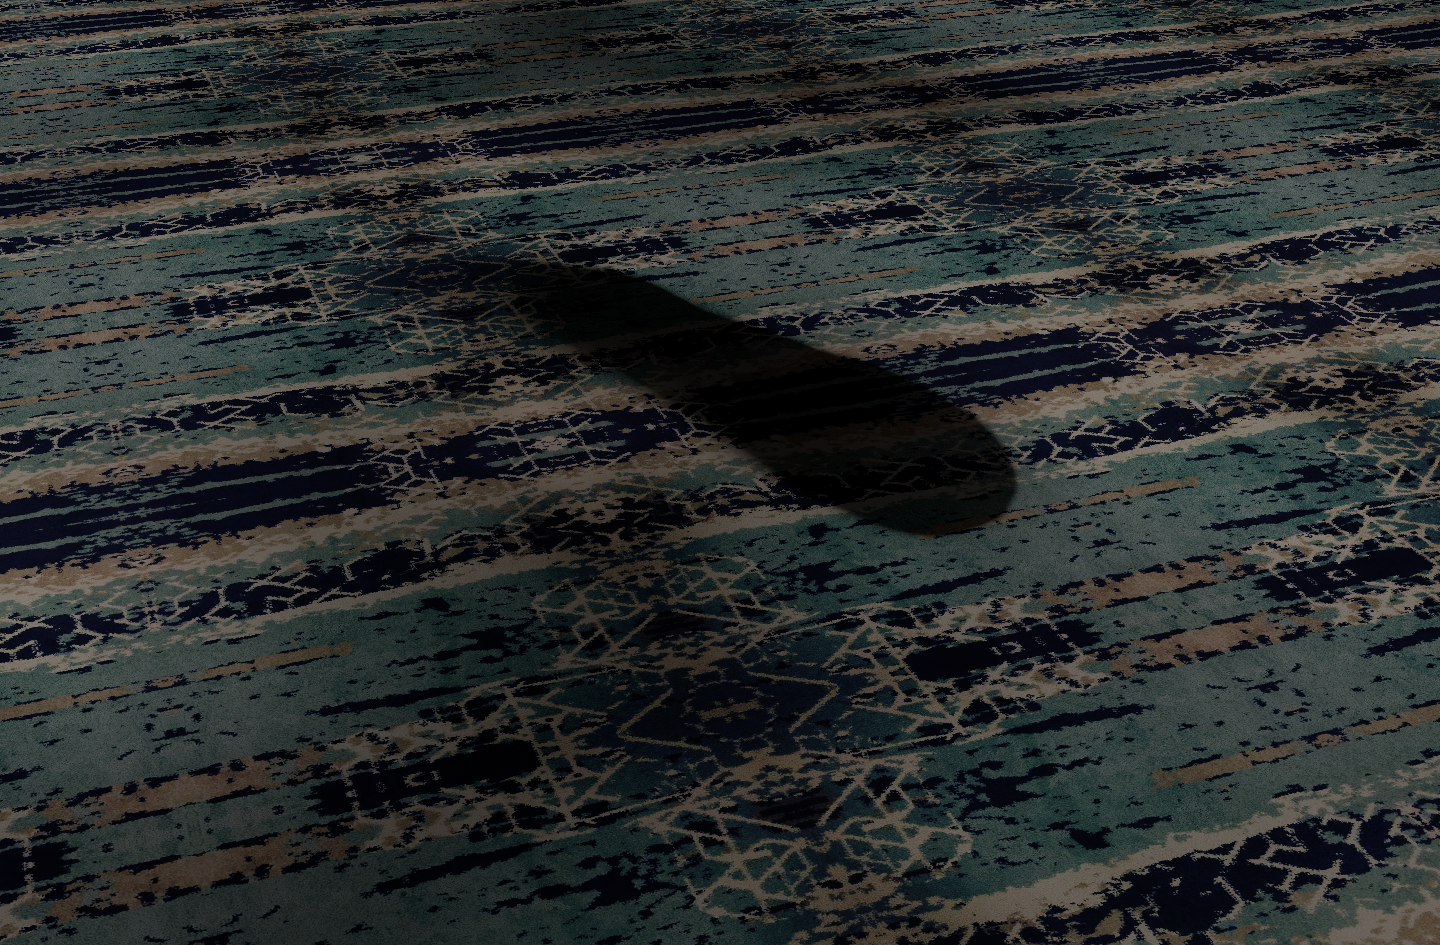
\includegraphics[width=\textwidth]{tilted_plan_and_shadow}
        \caption{Texture in scanner plane with added shadows}
        \label{fig:floor_in_plane}
    \end{subfigure}
    ~ %add desired spacing between images, e. g. ~, \quad, \qquad, \hfill etc. 
    %(or a blank line to force the subfigure onto a new line)
    \begin{subfigure}[b]{0.45\textwidth}
        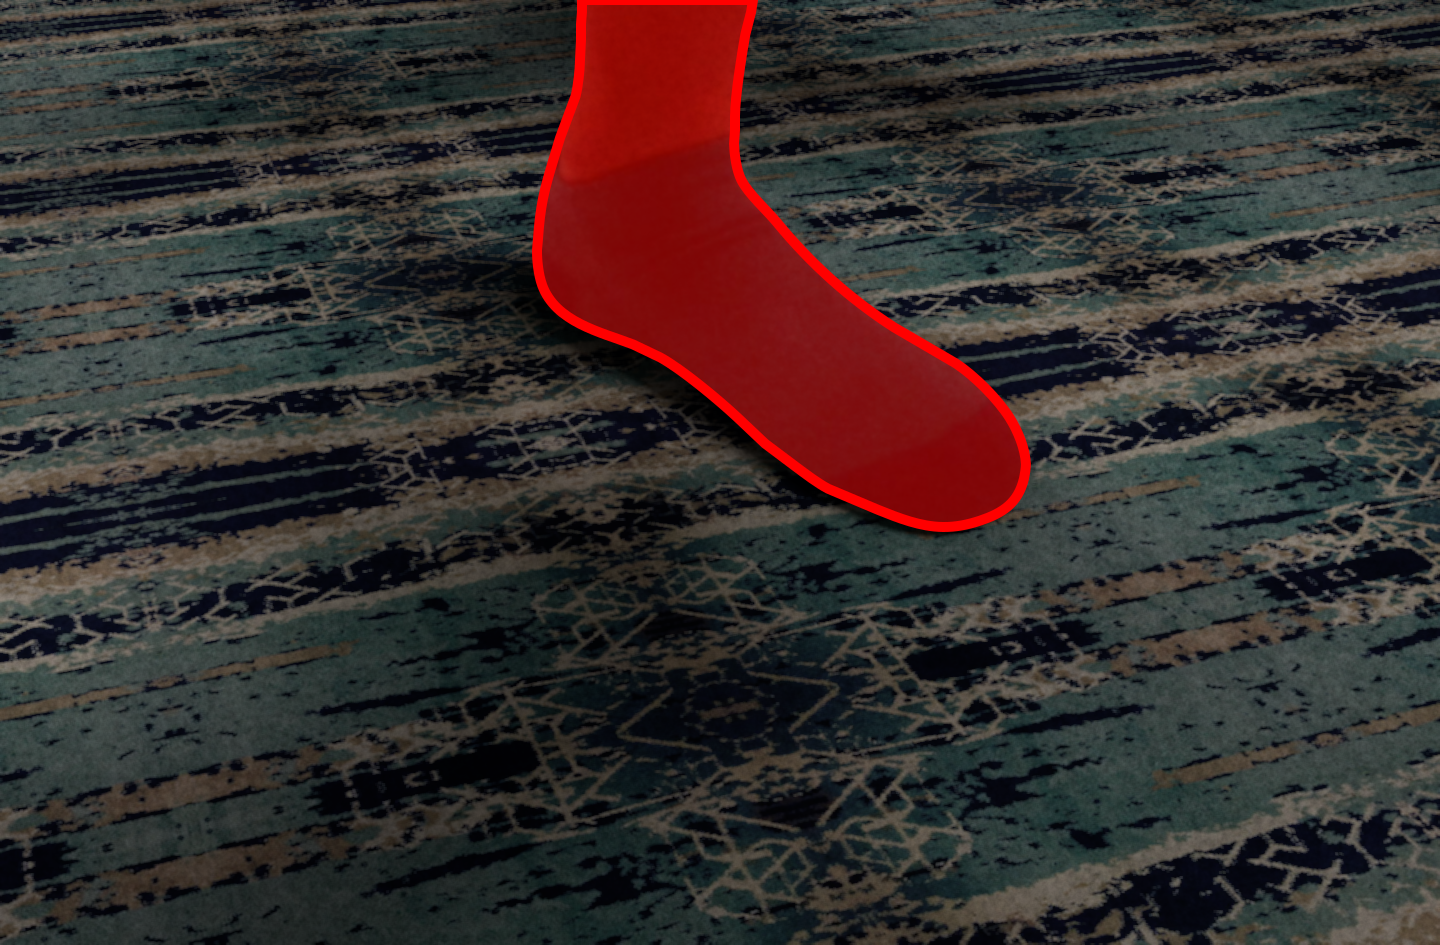
\includegraphics[width=\textwidth]{teleported_foot}
        \caption{The final image with segmentation}
        \label{fig:process_res}
    \end{subfigure}
    \caption{Steps for creating the synthetic data}\label{fig:process_synthetic}
\end{figure}

\begin{figure}[h]
  \centering
  \includegraphics[width=0.85\textwidth]{synthetic}
  \caption{Examples of images and segmentations from the synthetic dataset}
  \label{fig:data_synthetic}
\end{figure}

Secondly a dataset of 111 images taken of employees at \textit{Volumental} that
has been segmented by hand. This dataset is called \textit{real} and is
primarily used for testing how the methods generalize from  the synthetic data to
real images. Example images can be seen in \cref{fig:data_real}.

\begin{figure}[h]
  \centering
  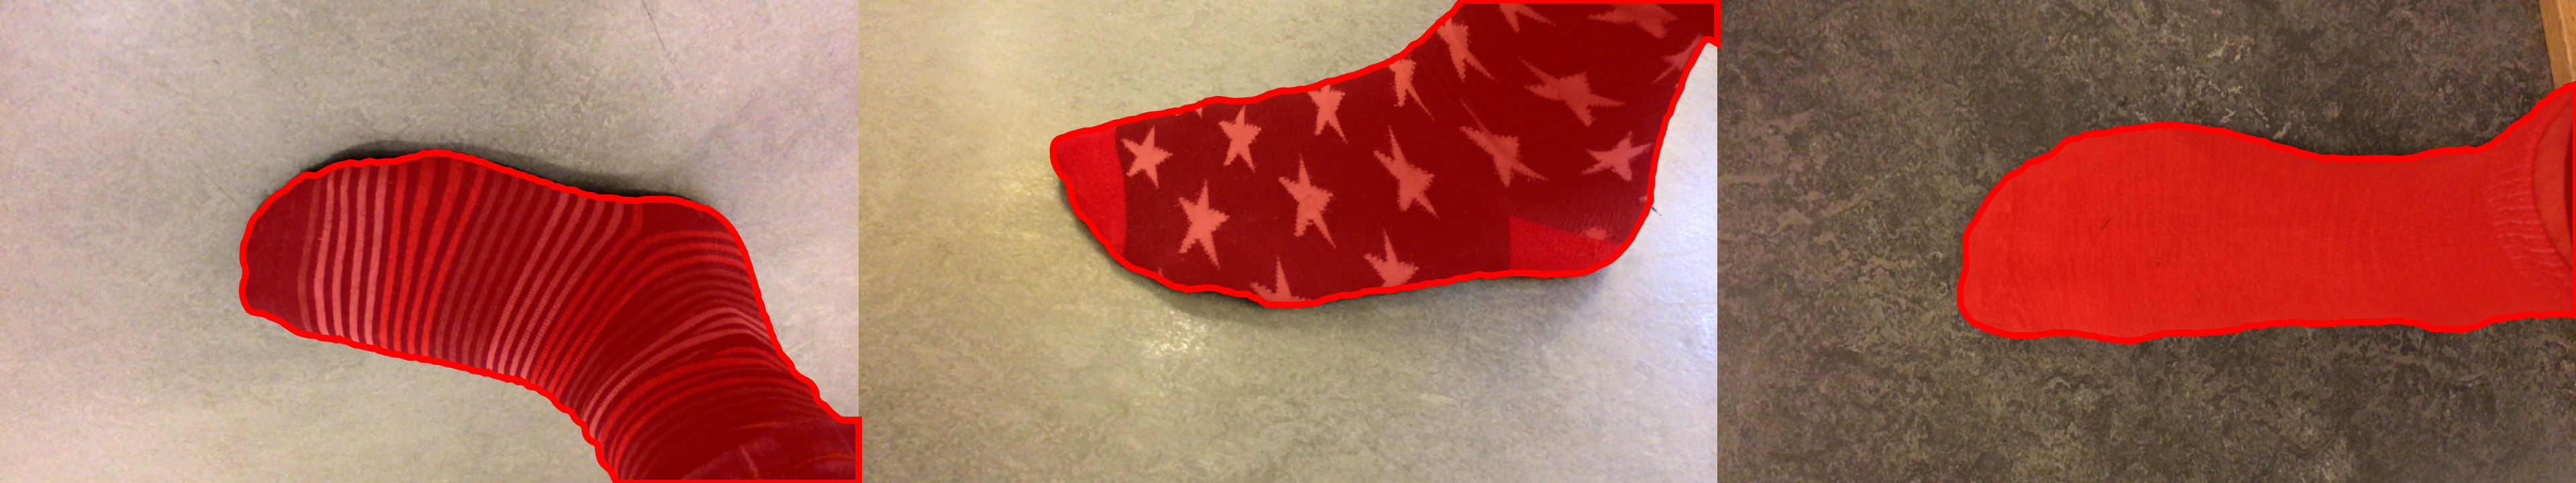
\includegraphics[width=0.85\textwidth]{real}
  \caption{Examples of images and segmentations from the real dataset}
  \label{fig:data_real}
\end{figure}

\subsection{Data augmentation}
One restriction with the \textit{synthetic} dataset is that, due to the
placement of the cameras, the images from the
scanner only come from four different angles. Fixed with regards to the
foot and all taken from approximately the same
distance. To enable the models to learn more general foot features despite
these restrictions the original images are augmented by dividing each image into
a \(3\times3\) grid, selecting a random point in each corner cell, and
performing an affine transformation to make these selected points the corners of
a new \(256\times256 \textit{px}\) image.

This augmentation introduces some random zoom, rotation, shear and translation
to the images and should hence help the algorithms learn generalizable features.
Some example of this can be seen in \cref{fig:augment}

\begin{figure}[h]
    \centering
    \begin{subfigure}[b]{0.3\textwidth}
        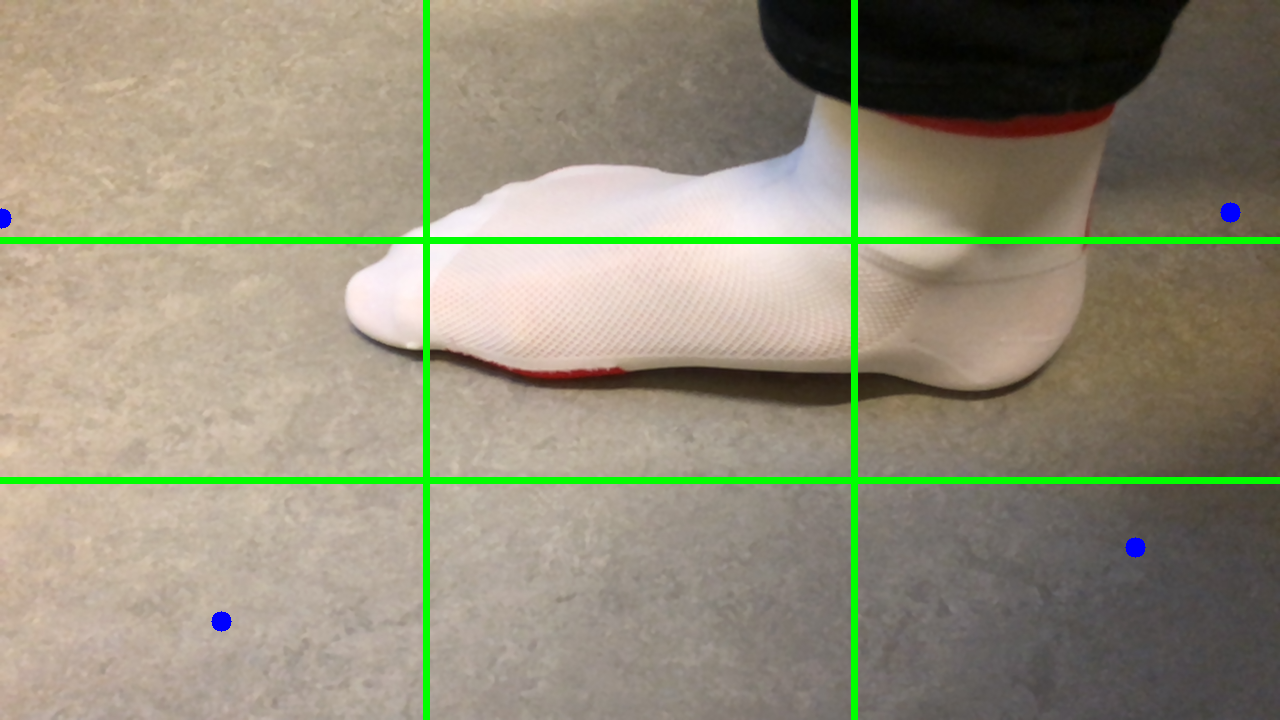
\includegraphics[width=\textwidth]{orig1}
    \end{subfigure}
    ~ %add desired spacing between images, e. g. ~, \quad, \qquad, \hfill etc. 
      %(or a blank line to force the subfigure onto a new line)
    \begin{subfigure}[b]{0.3\textwidth}
        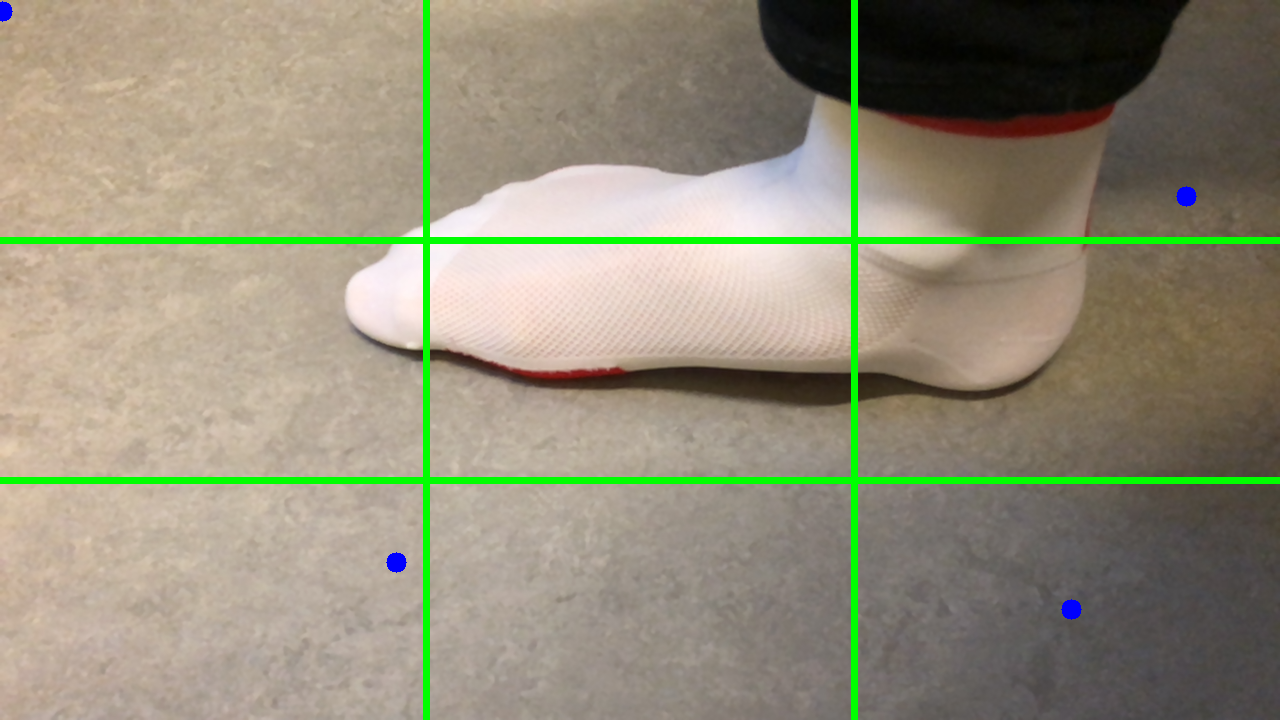
\includegraphics[width=\textwidth]{orig2}
      \end{subfigure}
    ~
    %add desired spacing between images, e. g. ~, \quad, \qquad, \hfill etc. 
    %(or a blank line to force the subfigure onto a new line)
    \begin{subfigure}[b]{0.3\textwidth}
        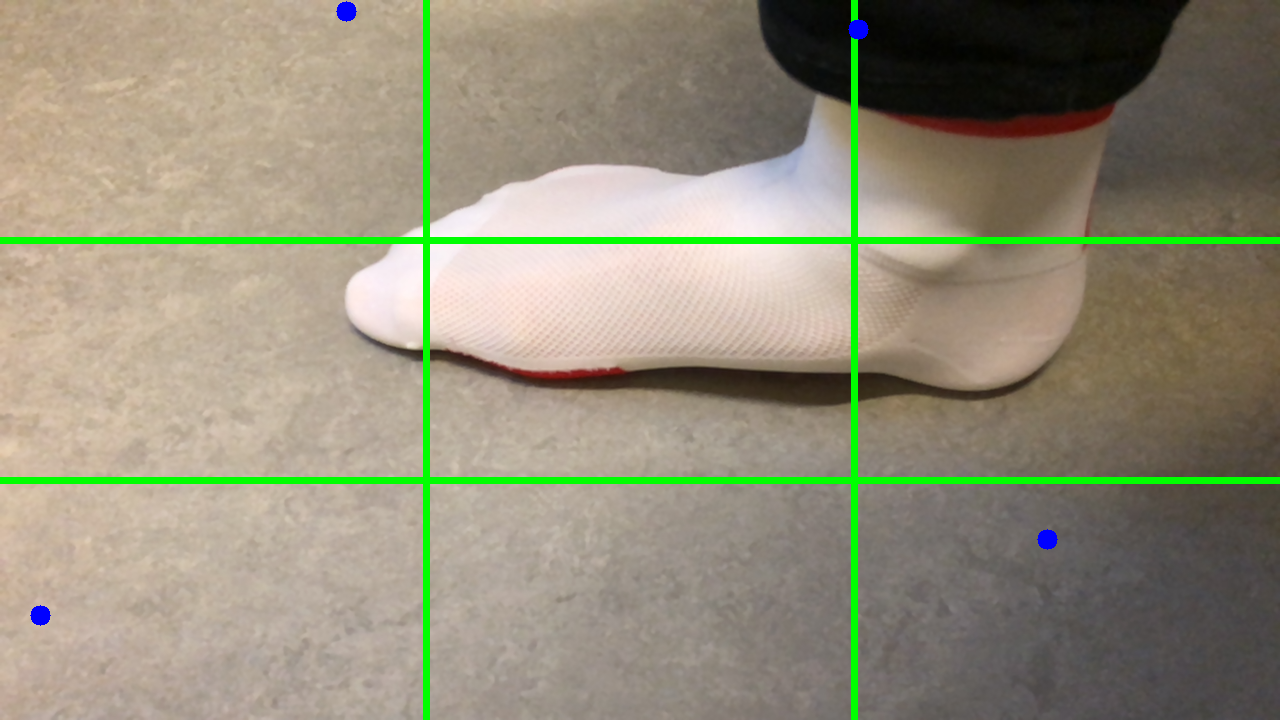
\includegraphics[width=\textwidth]{orig3}
      \end{subfigure}

      \begin{subfigure}[b]{0.3\textwidth}
        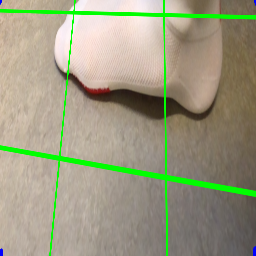
\includegraphics[width=\textwidth]{augmented1}
    \end{subfigure}
    ~ %add desired spacing between images, e. g. ~, \quad, \qquad, \hfill etc. 
      %(or a blank line to force the subfigure onto a new line)
    \begin{subfigure}[b]{0.3\textwidth}
        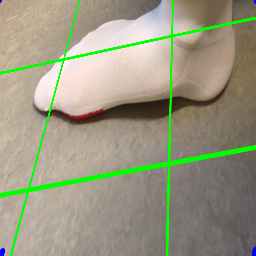
\includegraphics[width=\textwidth]{augmented2}
      \end{subfigure}
    ~
    %add desired spacing between images, e. g. ~, \quad, \qquad, \hfill etc. 
    %(or a blank line to force the subfigure onto a new line)
    \begin{subfigure}[b]{0.3\textwidth}
        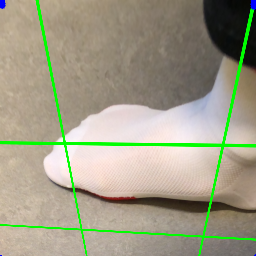
\includegraphics[width=\textwidth]{augmented3}
      \end{subfigure}
      \caption{Some random augmentations on the same image. Top row is the
        original image with the sampled corners are indicated in blue and
        the sample boundaries are indicated in green. Bottom row is the
        resulting image.}\label{fig:augment}
\end{figure}


\section{Network architectures}
For the experiments four different neural networks were evaluated against each
other. Details on each of these follow below. \todo{Gosh, this is not good at all...}

\subsection*{ENet}
This is a re-implementaiton of the \textit{ENet} architecture
\parencite{paszke2016enet} where the unpooling operations from the upsampling
blocks has been replaced with addition of the corresponding feature map from the
downsampling path due to restrictions in \textit{Keras}. An illustration of what
this means can be seen in \cref{fig:upscale}.

\begin{figure}[h]
  \centering
  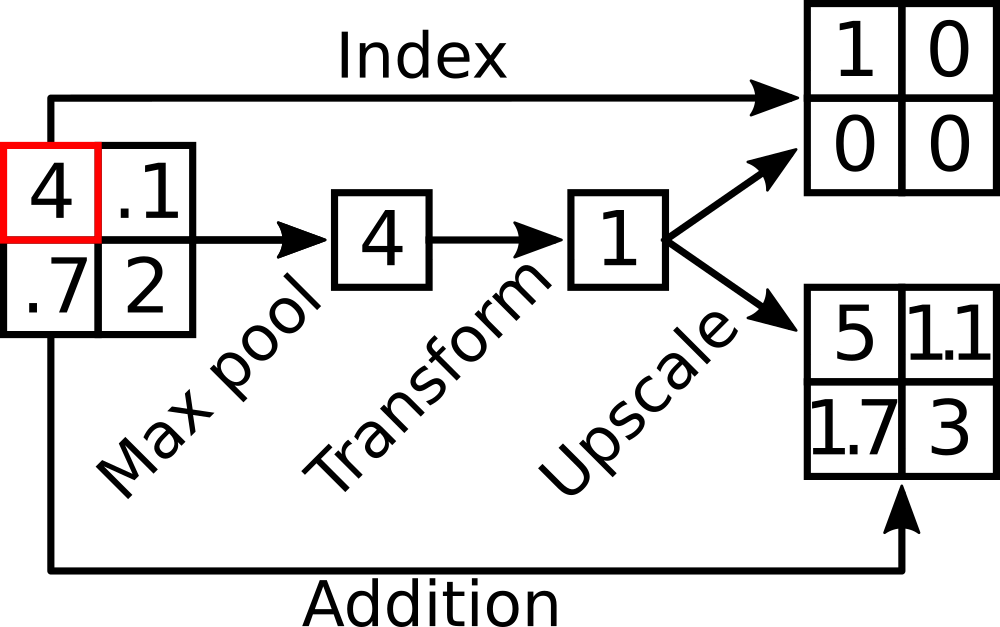
\includegraphics[width=0.5\textwidth]{upscale}
  \caption{A simple illustration of the difference between using the indices
    from max pooling (upper branch) and to add the feature map as it looked
    before max pooling (lower branch)
    to maintain image granularity during upsamlpling.}
  \label{fig:upscale}
\end{figure}

\subsection*{LinkNet}
This is a straight re-implementation of the LinkNet architecture \parencite{chaurasia2017linknet}.

\subsection*{MobileSeg}
This is a network for semantic segmentation that was built using the body of the
\textit{MobileNet} architecture \parencite{howard2017mobilenets} as the encoder of the network and then adds the
upsampling path from \textit{LinkNet} to this body and skip-connections are
introduced where the dimensions correspond to those in \textit{LinkNet}

\subsection*{FastLinkNet}
This network is designed as a hybrid between \textit{LinkNet} and
\textit{MobileNet} where the the layout of \textit{LinkNet} has been copied but
inspired by \textit{MobileNet} all the convolutions in the encoder blocks have
been replaced with depthwise separable convolutions, thus reducing model size
with approximately a factor \(4\).
Further inspiration was taken from the resolution
multiplier in the \textit{MobileNets} which is used to reduce the resolution of
the incoming image data to reduce the computation needed to process it by
downscaling the images by a factor \(2\) before segmentation and then bilineraly
upscaling the image to the full input size at the end.

\section{Loss functions}
To train the networks for semantic segmentation three different loss functions
were evaluated.

\subsection{Cross entropy}\label{section:cross_entropy}
The classical loss function for classification tasks is
\textit{Cross Entropy}.

\[\mathcal{L}_{CE}(Y, \hat{Y}) =- \sum_i Y_i \log\hat{Y_i}\]

Where \(Y\) is ground truth and \(\hat{Y}\) is the prediction and the index
\(i\) goes over all the pixels in the images. Since
semantic segmentation is the task of classifying each pixel in the image this is
a reasonable loss function.

\subsection{IoU loss}
In semantic segmentation a common performance measure is the intersect over union
\(IoU\) metric between the predicted segmentation and the ground truth.
\(IoU\) is defined as follows.
\[IoU = \frac{I}{U} = \frac{\textit{TP}}{\textit{FP} + \textit{TP} + \textit{FN}}\]
Where \(I\) is the intersect between the prediction and ground truth, \(U\) the union
between them and FP, FN, and TP indicate the false positive, false negative and
true positive respectively. These different quantities are illustrated in \cref{fig:IoU}.

This metric is used since it gives small objects as much weight as bigger ones.
This stands in comparison to using the proportion of correctly classified pixels
where classifying a image with a lot of background and a tiny foot as all background
would give good results.

\begin{figure}[h]
  \centering
  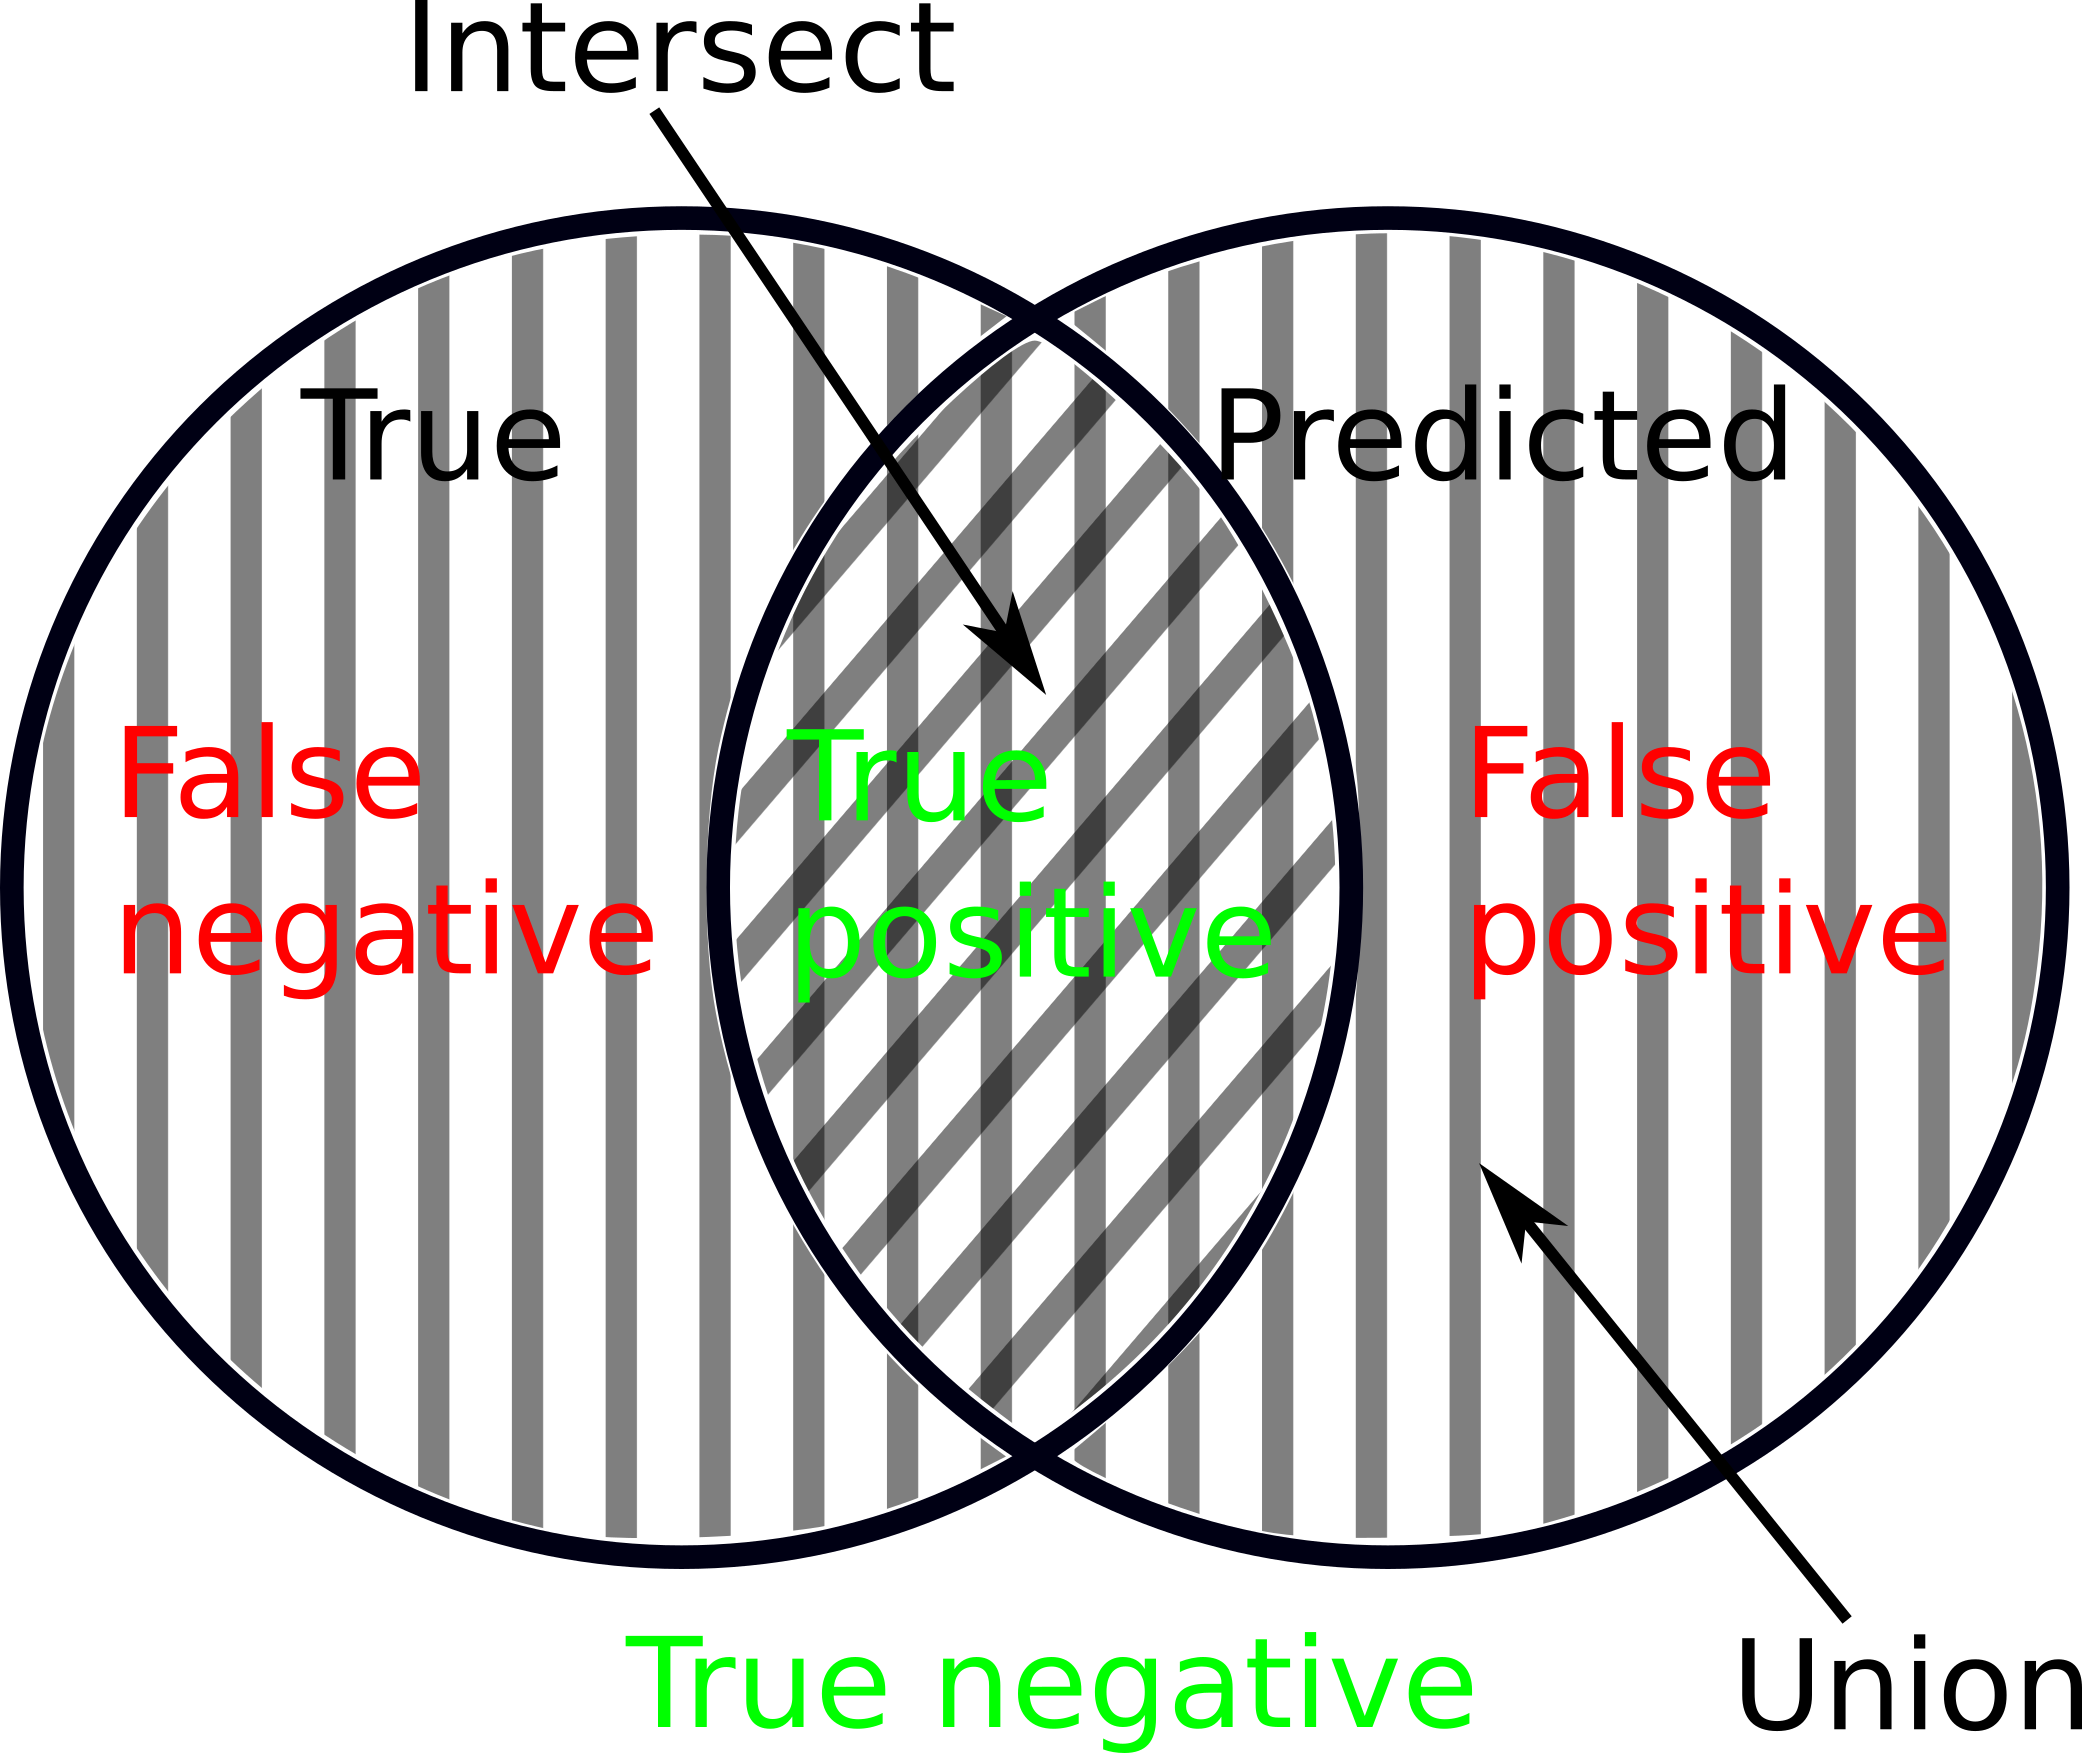
\includegraphics[width=0.40\textwidth]{IoU}
  \caption{Notation for \(IoU\)}
  \label{fig:IoU}
\end{figure}


To directly optimize for \(IoU\) \textcite{rahman2016optimizing} introduced
a \(IoU\) loss.
\[\mathcal{L}_{IoU} = 1 - IoU\]

If we now let \(V = {1, 2, \dots, N}\) be the set of pixels in the image, \(\hat{Y}\)
the softmax outputs from the network at each pixel and \(Y\) the ground truth
segmentation. The intersection \(I(\hat{Y})\) and union \(U(\hat{Y})\) can be
approximated with the following:

\[I(\hat{Y}) = \sum_{v \in V} Y_v \odot \hat{Y_v}\]
\[U(\hat{Y}) = \sum_{v \in V}\left( Y_v + \hat{Y_v} - Y_v \odot \hat{Y_v} \right) \]

Where \(\odot\) represents the element-wise Hadamard product.

The \(IoU\) loss hence becomes

\[\mathcal{L}_{IoU} = 1 - \frac{I(\hat{Y})}{U(\hat{Y})}\]


\subsection{Distillation}
% \todo{Write a bit about distillation}
When training using distillation loss \parencite{hinton2015distilling} a large
previously trained network is used to help guide the student model during
training. The loss function here is defined as:

\[\mathcal{L}_{distillation} = \mathcal{L}_{CE}(Y, \hat{Y}) + \lambda T^2\mathcal{L}_{CE}(\hat{Y}^*, \hat{Y}_{teacher}^*)\]

Where \(\mathcal{L}_{CE}\) is the cross entropy loss from
\cref{section:cross_entropy} and \(\hat{Y}^*\) and \(\hat{Y}^*_{teacher}\) are the softened,
high temperature softmax outputs, see \cref{fig:softmax} from the student and teacher networks
respectively. \(\lambda\) is the mixing factor controlling how much influence
should come from the hard ground truth and how much should come from the soft
student-teacher training. \(T\) is the temperature with which the softmax were softened and
it is used to compensate for the fact that the gradient with respect to the soft
loss decreases with a factor \(\frac{1}{T^2}\) as explained in the initial
paper \parencite{hinton2015distilling}. The high temperature softmax is defined
as follows: 

\[\hat{Y}_i^* = \frac{e^{a_i/T}}{\sum_j e^{a_j/T}}\]

Here \(a\) are the activations from the preceding layer and \(T\) is the
temperature. If \(T = 1\) we get the normal softmax values and if \(T > 0\) we
get a softer output distribution making it easier for the student to learn from
the low probability classes of the teacher. 

\begin{figure}[h]
    \centering
    \begin{subfigure}[b]{0.3\textwidth}
        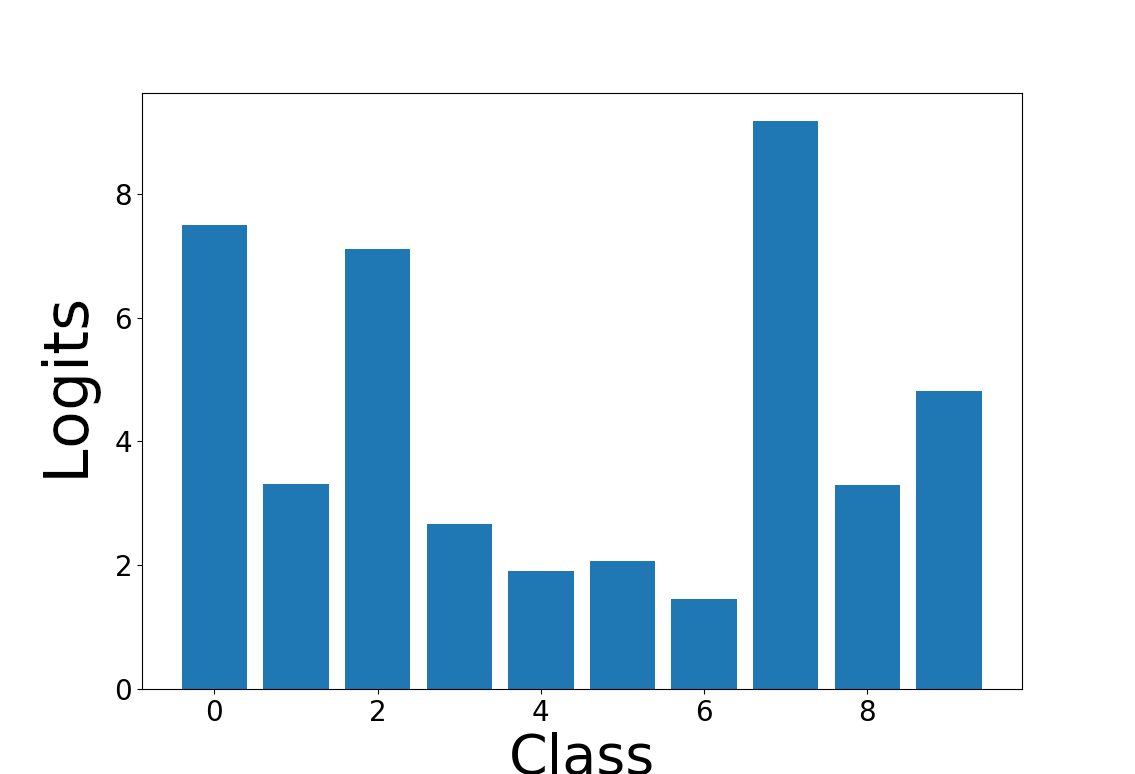
\includegraphics[width=\textwidth]{softmax_in}
        \subcaption{Log-likelihood}
    \end{subfigure}
    ~ %add desired spacing between images, e. g. ~, \quad, \qquad, \hfill etc. 
      %(or a blank line to force the subfigure onto a new line)
    \begin{subfigure}[b]{0.3\textwidth}
        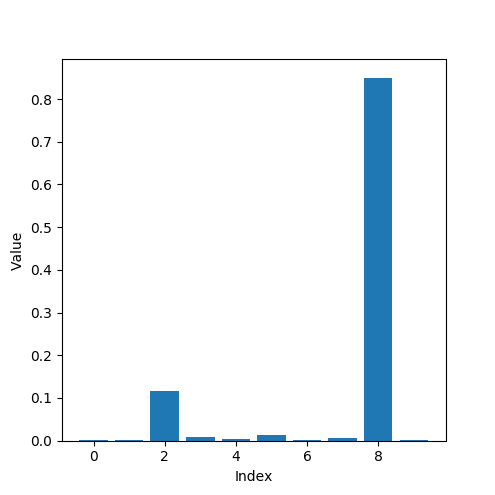
\includegraphics[width=\textwidth]{softmax_t1}
        \subcaption{Normal softmax}
      \end{subfigure}
    ~
    %add desired spacing between images, e. g. ~, \quad, \qquad, \hfill etc. 
    %(or a blank line to force the subfigure onto a new line)
    \begin{subfigure}[b]{0.3\textwidth}
        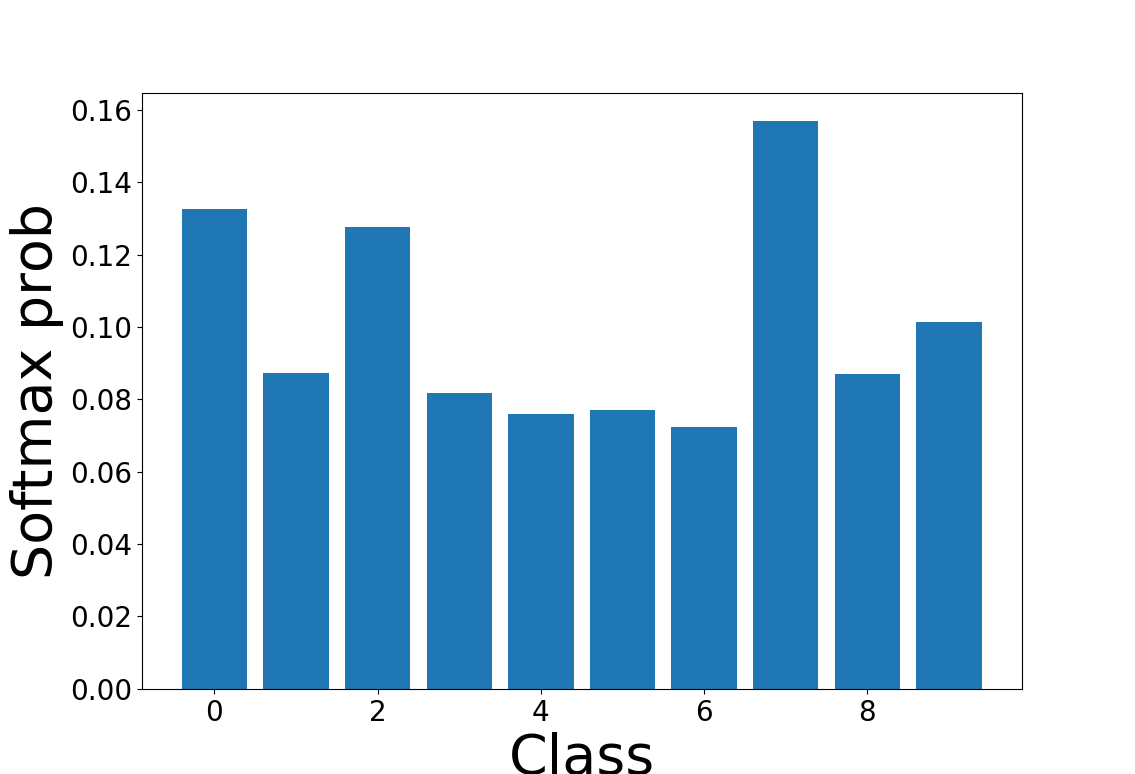
\includegraphics[width=\textwidth]{softmaxT10}
        \subcaption{Softmax, \(T=10\)}
      \end{subfigure}
     \caption{An illustaration of softmax using different temperatures, to the
       left is the input, in the middle output from \(T=1\) softmax and to the
       right \(T = 10\)}\label{fig:softmax}
\end{figure}


\chapter{Experiment}
To test the suitability of the different models and loss functions presented in
\cref{chap:method} they were trained and evaluated. The training procedure and
the different performance metrics used will be presented in the following
sections.

\section{Training}
% \todo{Gör detta till typ ett stycke om optimering, ett om hyper}
% The networks were defined and trained in \textit{Keras} \parencite{keras} using the
% \textit{tensorflow} \parencite{tensorflow} backend, enabling easy
% experimentation and fast execution on the GPUs available. Hyperparameter
% optimization was handled by the \textit{hyperopt} \parencite{hyperopt} package which worked neatly
% along with the other frameworks.

% Training was run for \(50\) epochs of \(50\) steps each with a batch size of \(32\).
% \(ADAM\) \parencite{ADAM} was used as the optimizer and hyperparameter
% optimization was run for 100 iterations of random search in the search space
% \(0.000001 < \eta < 0.01\), \( 0 < p_{dropout} < 1\), \(f_{loss} \in \{L_{CE},
% L_{IoU}, L_{distillation}\}\). And \( 1 < T < 100\), \(0< \lambda <10\) when
% distillation loss is used. 

The networks were defined and trained in \textit{Keras} \parencite{keras} using the
\textit{tensorflow} \parencite{tensorflow} backend. This framework enabled easy
experimentation and fast execution on the GPUs available, a \textit{GeForce GTX
  1080 Ti} and a \textit{GeForce GTX TITAN}. For training the networks the
\textit{ADAM} optimizer\parencite{ADAM}, an adaptive extension to stochastic
gradient decent that has become very popular in the deep learning community, was
used. Training was run for 50 epochs each consisting of 50 steps with a batch
size of \(32\). The training partition of the synthetic dataset is used for
training and the loss on the validation set is monitored and the learning rate
reduced by a factor 10 if validation doesn't decrease for \(3\) epochs.

In this training a bunch of hyperparameters have to be chosen beforehand. To
determine good values for some of the most important of these, namely
learning rate \(\lambda\), the dropout probability \(p_{dropout}\), the
loss function \(\mathcal{L}\), and the parameters of distillation loss
temperature \(T\) and mixing factor \(\lambda\) hyperparameter optimization is
used. This means that the entire training procedure was run \(100\) times, each
time with the hyperparameters randomly sampled from search space in
\cref{tab:search_space} and the performance on the validation set is monitored
for these runs. This means that we can find the settings that give the optimal
performance. Hyperparameter optimization was facilitated by the python package
\textit{hyperopt} \parencite{hyperopt}.

\begin{table}[]
\centering
\caption{The search space used in hyper parameter optimization. The temperature
  \(T\) and the mixing factor \(\lambda\) are only relevant when the loss
  function \(\mathcal{L} = \mathcal{L}_{distiallation}\).}
\label{tab:search_space}
\begin{tabular}{@{}ll@{}}
\toprule
Hyper parameter     & Search space \\ \midrule
Learning rate \(\eta\)      &      \(0.000001 < \eta < 0.01\)        \\
Dropout \(p_{dropout}\)&  \( 0 < p_{dropout} < 1\)            \\
Loss function \(\mathcal{L}\)    &    \(\mathcal{L} \in \{L_{CE},L_{IoU}, L_{distillation}\}\)          \\
Temperature \(T\)        &      \( 1 < T < 100\)        \\
Mixing factor \(\lambda\)      &     \(0< \lambda <10\)         \\ \bottomrule
\end{tabular}
\end{table}

\section{Evaluation}
When evaluating the models two major things are of interest for this work.
Firstly, how accurate the models are, how well they perform the prediction task.
Secondly, How efficient the models are, how well they can be run on mobile
hardware. A good balance between these two is necessary, the models are useless
if they give perfect segmentations but takes seconds to do so for a single frame
or can't fit on a smartphone. Likewise, models that can be reliably run at 20
fps but that give results comparable to random are also useless. The metrics
used to quantify how well the models perform both of these tasks will be
presented in the following sections.

\subsection{Accuracy measures}
To compare the predicted segmentations from the models to the ground truth data
and quantify how well they correspond a lot of different accuracy measures can
be used. A few of these different measures are presented in the following
sections. For the experiments these different measures have been calculated on
both the held out test set of the synthetic dataset and the dataset of real
images.

\subsubsection{Mean accuracy}

\subsubsection{IoU}

\subsection{Efficiency measures}
To evaluate the degree to which the models can be run on a smartphone they were
tested on a \textit{ZTE Axon 7} android phone using \textit{tensorflows}
benchmarking tools. From this inference time, and number of Floating point
operations (\textit{FLOPs}) calculated for inference was extracted. The size
required to store the models was also measured. 

\chapter{Results}
\todo{nått om olika loss functions}
The resulting segmentations from the best trained models of each architecture
can be seen for the real dataset in \cref{fig:seg_real} and for the synthetic
data set in \cref{fig:seg_test}. The mean pixel accuracy and IoU metrics
achieved by the models on the test set of the synthetic dataset and the real
dataset can be seen in \cref{tab:res_performance} and the results from the
benchmarks on the models are listed in \cref{tab:res_resources}.
\begin{figure}[h]
  \centering
  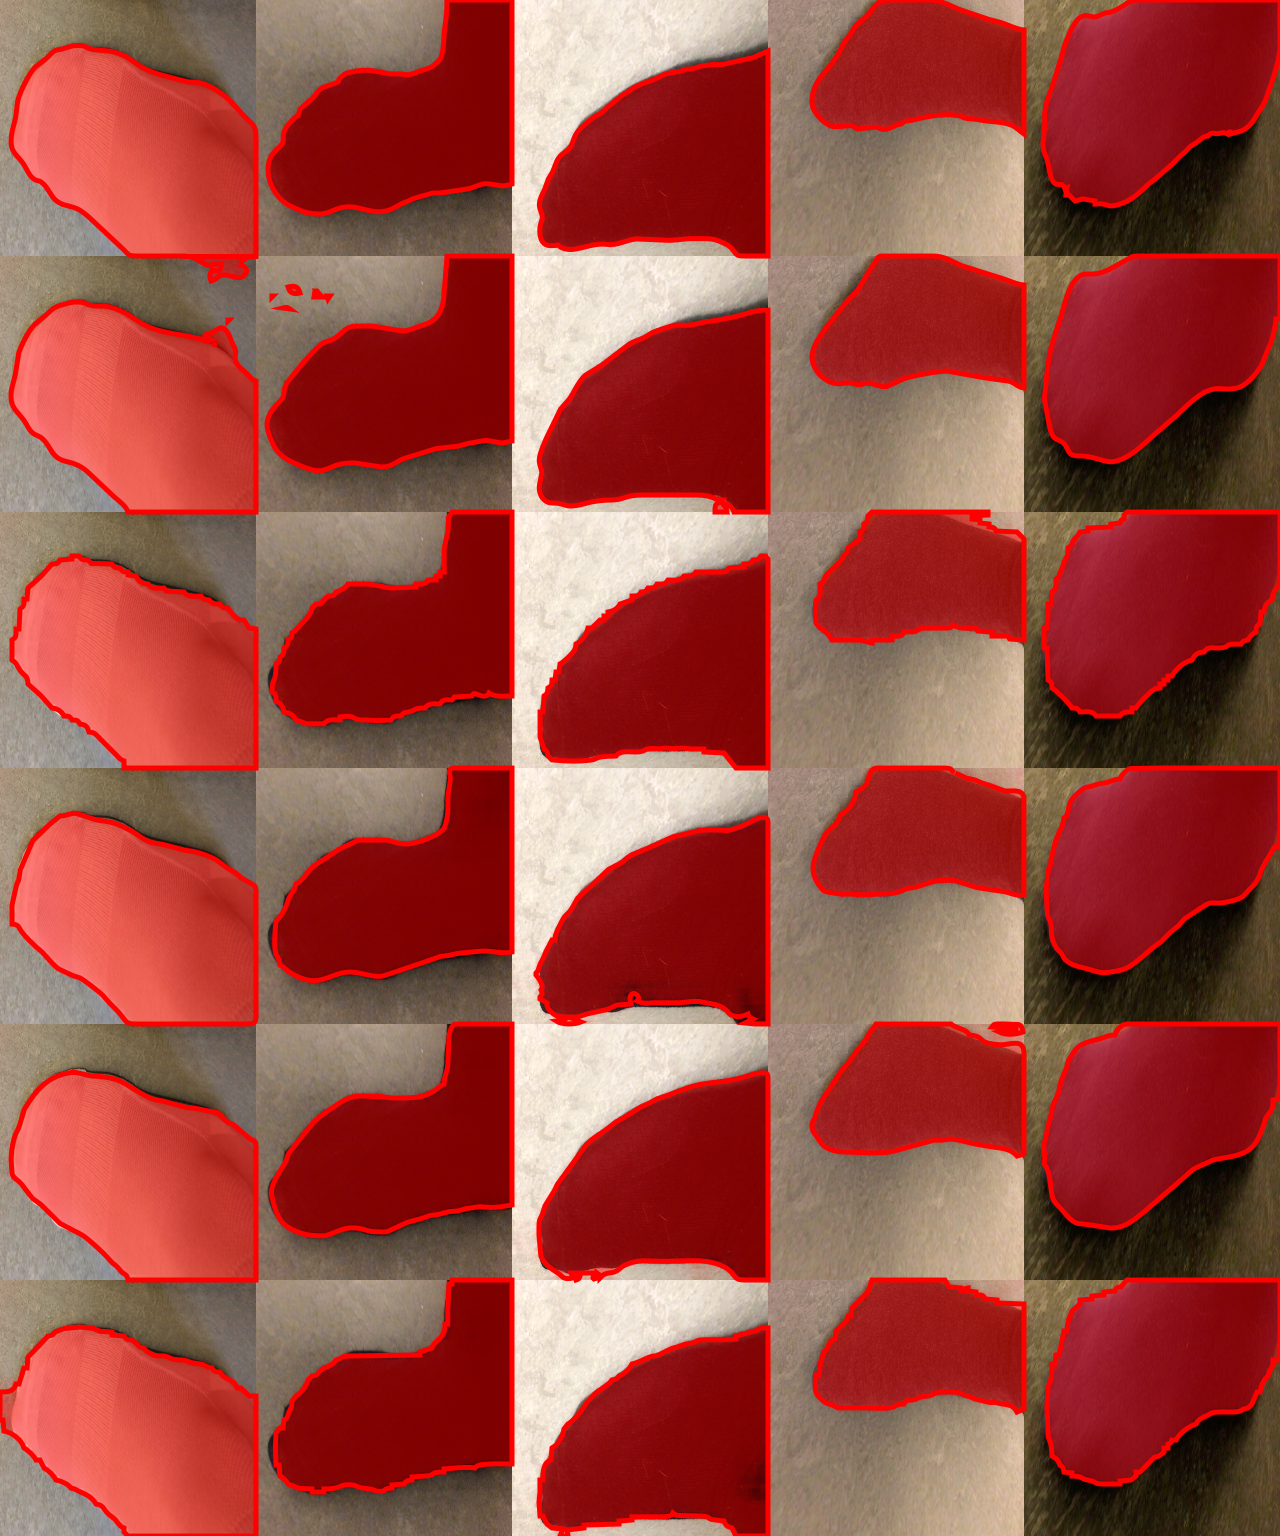
\includegraphics[width=\textwidth]{real_color}
  \caption{Resulting segmentations on the real dataset from the different models. First row is the ground
    truth, below that EmilSeg, ENet, LinkNet, MobileSeg, and FastLinkNet.}
  \label{fig:seg_real}
  \end{figure}

 \begin{figure}[h]
  \centering
  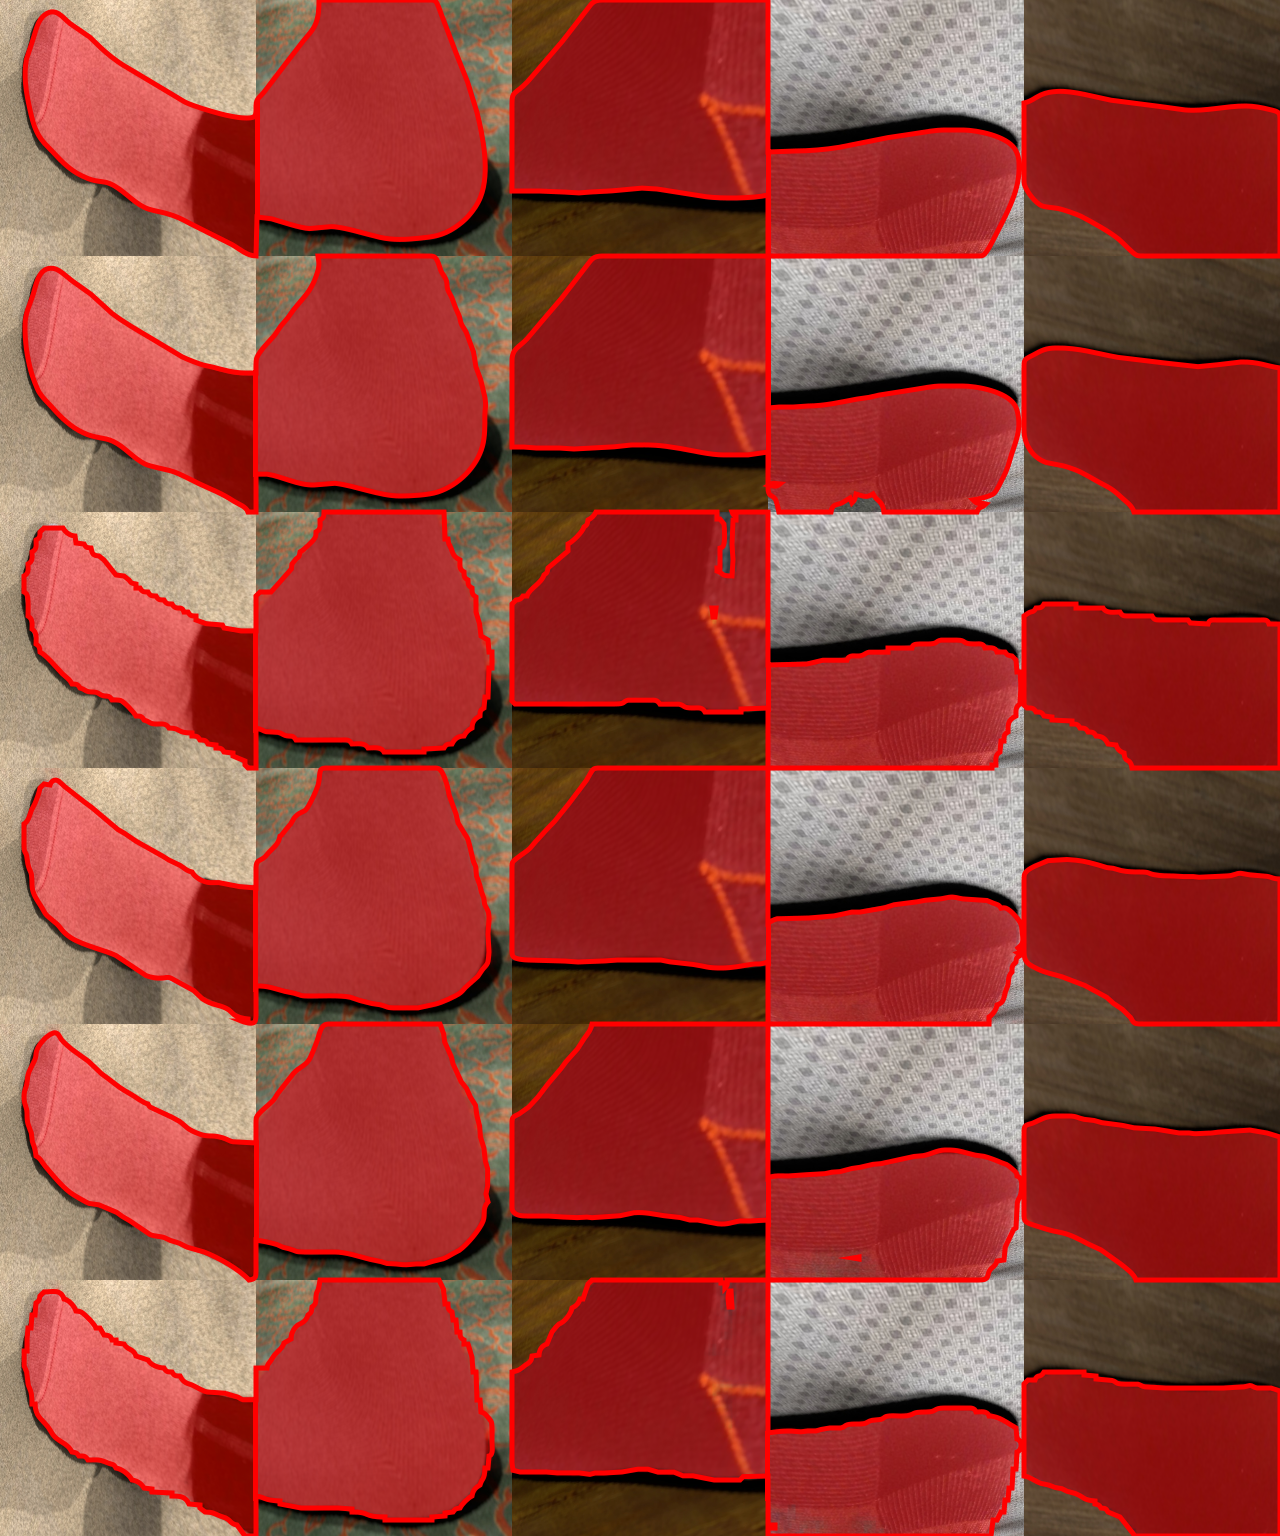
\includegraphics[width=\textwidth]{test_color}
  \caption{Resulting segmentations on the test set of the synthetic dataset from the different models. First row is the ground
    truth, below that EmilSeg, ENet, LinkNet, MobileSeg, and FastLinkNet.}
  \label{fig:seg_test}
  \end{figure}
  
\begin{table}[]
\centering
\caption{Comparison of size, FLOPs and time required for inference of the
  different models. Timing was done on a \textit{ZTE Axon 7} android smartphone.}
\label{tab:res_resources}
\begin{tabular}{@{}lllll@{}}
\toprule
Model       &  GFLOPs  & Inference time {[}ms{]} & Size {[}Mb{]}  \\ \midrule
EmilSeg     &  55.37   & 4439                    & 85             \\
ENet        &  10.38   & 1045                    & 1.4            \\
LinkNet     &  1.75    & 234                     & 45             \\
MobileSeg   &  2.68    & 555                     & 18             \\
FastLinkNet &  0.287   & 73                      & 7.2            \\ \bottomrule
\end{tabular}
\end{table}

\begin{table}[]
\centering
\caption{Comparison of the test performance between the different models}
\label{tab:res_performance}
\begin{tabular}{@{}llllll@{}}
\toprule
Model       & Test accuracy & Test IoU & Real accuracy & Real IoU \\ \midrule
EmilSeg    & 0.9912 & 0.9860 & 0.9740 & 0.9814 \\
ENet       & 0.9774 & 0.9116 & 0.9738 & 0.9117 \\
LinkNet    & 0.9797 & 0.9141 & 0.9724 & 0.9145 \\
MobileSeg  & 0.9834 & 0.9146 & 0.9744 & 0.9144 \\ 
FastLinkNet& 0.9797 & 0.9153 & 0.9707 & 0.9148 \\  \bottomrule
\end{tabular}
\end{table}

\chapter{Discussion}
The fastest network produced, \textit{FastLinkNet}, runs inference in \(73 ms\)
\cref{tab:res_resources}, enabling frame rates of over \(10fps\) on a smartphone
from \(2016\) without the use of hardware acceleration on GPU or digital signal
processor (DSP) which are both
expected features as the mobile neural network platforms mature.
Moreover the resulting segmentations from \textit{FastLinkNet} look good on both
the synthetic, \cref{fig:seg_test}, and the real dataset, \cref{fig:seg_real}, meaning that
the models are usable in real time right now and that significant performance
boosts could be expected in the near future.

From \cref{tab:res_performance} it is interesting to note that all of the
trained networks perform almost the same and very close to the big baseline
model \textit{EmilSeg}. This might be due to the fact that the datasets contain
too little complexity and hence present a rather easy problem for
the models. Some tests from running the models on a smartphone and testing it
out in real world applications seem to support this since the model really
struggles to handle complex scenes, multiple feet in the image, differing image
scales, bare feet etc. Some tests of this can be seen in \cref{chapter:real_world}.
It is also noteworthy that the performance on the real and the synthetic
datasets are almost identical for all the models except for \textit{EmilSeg}
indicating that generalization between the datasets works really well.

\section{Further work}
The teacher model \textit{EmilSeg} in distillation
was not subjected to extensive hyperparameter optimization and was not
necessarilly trained to full convergence meaning that distillation could get
better results if more time was spent on tweeking not only the students but
also the teacher.

Further performance could also be gained from not just using the the current
frame for segmentation but the entire stream of information. This could for
example be done by adding a long short-term memory (LSTM) cell to the
bottlenecks of the segmentation networks or by feeding the predicted
segmentation at each frame back as a fourth channel in the input for the next
frame. These approaches however would require segmented video data for training
or heavy augmentation of the existing images to produce plausible fake video
from still images. An other issue with these approaches is also that they can
add a lot of computational overhead to the models and hence slow down execution to an
unacceptable degree.

An approach to getting better and more reliable results from the networks that
would not slow down execution would be to rethink the training process. For
example pre training the encoder on \textit{ImageNet} or the entire network on
an other segmentation dataset like \textit{CamVid} could improve performance. To
get more plausible segmentations from the networks they could also be trained as
a generative adversarial network
(GAN) as proposed by \textcite{AdverserialSegmentation}.

The quality of the synthetic dataset could also be improved, either by training a
\textit{GAN} to produce the training images or by using the full 3D-models of
the feet from the scanner, mapping the texture from the images back to this model
and then placing the foot at an arbitrary angle and distance from the virtual
camera. Giving a greater variance in the data.

\section{Impact}
When handling data like images of feet in this fashion the question of privacy
is always relevant and being careful about anonymising data is important.
Further, the aim of this work is to automate away sales clerks and instead
giving that experience online. This overall trend of automating away work is
bound make some people unemployed and a serious discussion about how this
situation about how this unemployability is to be handled in society is well
overdue. However, a online shopping experience where a good fit is acquired at
first try is going to reduce returns and in turn shipping and the carbon
footprint of online retail overall. 

On a more technical level the same methods that help reduce the power required
and computational resources needed for running neural networks on smartphones
are being applied to larger systems as well. This reduces the energy consumption
of machine learning models that are becoming more and more prominent in our
lives and helps reduce the power requirements of the industry overall.

\printbibliography[heading=bibintoc]% Print the bibliography (and make it appear in the table of contents)

\appendix

\chapter{Real world tests} \label{chapter:real_world}
\todo{add a capture image button to the app and go out in the world and take
  some cool images}


\end{document}
